
%% bare_jrnl.tex
%% V1.3
%% 2007/01/11
%% by Michael Shell
%% see http://www.michaelshell.org/
%% for current contact information.
%%
%% This is a skeleton file demonstrating the use of IEEEtran.cls
%% (requires IEEEtran.cls version 1.7 or later) with an IEEE journal paper.
%%
%% Support sites:
%% http://www.michaelshell.org/tex/ieeetran/
%% http://www.ctan.org/tex-archive/macros/latex/contrib/IEEEtran/
%% and
%% http://www.ieee.org/



% *** Authors should verify (and, if needed, correct) their LaTeX system  ***
% *** with the testflow diagnostic prior to trusting their LaTeX platform ***
% *** with production work. IEEE's font choices can trigger bugs that do  ***
% *** not appear when using other class files.                            ***
% The testflow support page is at:
% http://www.michaelshell.org/tex/testflow/


%%*************************************************************************
%% Legal Notice:
%% This code is offered as-is without any warranty either expressed or
%% implied; without even the implied warranty of MERCHANTABILITY or
%% FITNESS FOR A PARTICULAR PURPOSE! 
%% User assumes all risk.
%% In no event shall IEEE or any contributor to this code be liable for
%% any damages or losses, including, but not limited to, incidental,
%% consequential, or any other damages, resulting from the use or misuse
%% of any information contained here.
%%
%% All comments are the opinions of their respective authors and are not
%% necessarily endorsed by the IEEE.
%%
%% This work is distributed under the LaTeX Project Public License (LPPL)
%% ( http://www.latex-project.org/ ) version 1.3, and may be freely used,
%% distributed and modified. A copy of the LPPL, version 1.3, is included
%% in the base LaTeX documentation of all distributions of LaTeX released
%% 2003/12/01 or later.
%% Retain all contribution notices and credits.
%% ** Modified files should be clearly indicated as such, including  **
%% ** renaming them and changing author support contact information. **
%%
%% File list of work: IEEEtran.cls, IEEEtran_HOWTO.pdf, bare_adv.tex,
%%                    bare_conf.tex, bare_jrnl.tex, bare_jrnl_compsoc.tex
%%*************************************************************************

% Note that the a4paper option is mainly intended so that authors in
% countries using A4 can easily print to A4 and see how their papers will
% look in print - the typesetting of the document will not typically be
% affected with changes in paper size (but the bottom and side margins will).
% Use the testflow package mentioned above to verify correct handling of
% both paper sizes by the user's LaTeX system.
%
% Also note that the "draftcls" or "draftclsnofoot", not "draft", option
% should be used if it is desired that the figures are to be displayed in
% draft mode.
%

\documentclass[journal]{IEEEtran}
%\documentclass[11pt, draftcls, onecolumn]{IEEEtran}

% Single column review mode:
%\documentclass[12pt,journal,onecolumn]{IEEEtran}
%\newcommand\CLASSINPUTbaselinestretch{2}
%\RequirePackage{calc}
%\RequirePackage{fp} 
% Left margin = 1 inch + hoffset + oddsidemargin (or evensidemargin)
% Adding the 2cm gutter width to the odd/even side margins:
%\setlength\hoffset{0pt}
%\setlength\oddsidemargin{4cm}       % 4cm margins on the left side
%\addtolength\oddsidemargin{-1in}    % Subtract the initial 1 inch
%\setlength\textwidth{21cm-8cm}    % A4 width (21cm) minus margins on either side

%
% If IEEEtran.cls has not been installed into the LaTeX system files,
% manually specify the path to it like:
% \documentclass[journal]{../sty/IEEEtran}





% Some very useful LaTeX packages include:
% (uncomment the ones you want to load)


% *** MISC UTILITY PACKAGES ***
%
%\usepackage{ifpdf}
% Heiko Oberdiek's ifpdf.sty is very useful if you need conditional
% compilation based on whether the output is pdf or dvi.
% usage:
% \ifpdf
%   % pdf code
% \else
%   % dvi code
% \fi
% The latest version of ifpdf.sty can be obtained from:
% http://www.ctan.org/tex-archive/macros/latex/contrib/oberdiek/
% Also, note that IEEEtran.cls V1.7 and later provides a builtin
% \ifCLASSINFOpdf conditional that works the same way.
% When switching from latex to pdflatex and vice-versa, the compiler may
% have to be run twice to clear warning/error messages.






% *** CITATION PACKAGES ***
%
\usepackage{cite}
% cite.sty was written by Donald Arseneau
% V1.6 and later of IEEEtran pre-defines the format of the cite.sty package
% \cite{} output to follow that of IEEE. Loading the cite package will
% result in citation numbers being automatically sorted and properly
% "compressed/ranged". e.g., [1], [9], [2], [7], [5], [6] without using
% cite.sty will become [1], [2], [5]--[7], [9] using cite.sty. cite.sty's
% \cite will automatically add leading space, if needed. Use cite.sty's
% noadjust option (cite.sty V3.8 and later) if you want to turn this off.
% cite.sty is already installed on most LaTeX systems. Be sure and use
% version 4.0 (2003-05-27) and later if using hyperref.sty. cite.sty does
% not currently provide for hyperlinked citations.
% The latest version can be obtained at:
% http://www.ctan.org/tex-archive/macros/latex/contrib/cite/
% The documentation is contained in the cite.sty file itself.






% *** GRAPHICS RELATED PACKAGES ***
%
\ifCLASSINFOpdf
  % \usepackage[pdftex]{graphicx}
  % declare the path(s) where your graphic files are
  % \graphicspath{{../pdf/}{../jpeg/}}
  % and their extensions so you won't have to specify these with
  % every instance of \includegraphics
  % \DeclareGraphicsExtensions{.pdf,.jpeg,.png}
\else
  % or other class option (dvipsone, dvipdf, if not using dvips). graphicx
  % will default to the driver specified in the system graphics.cfg if no
  % driver is specified.
  % \usepackage[dvips]{graphicx}
  % declare the path(s) where your graphic files are
  % \graphicspath{{../eps/}}
  % and their extensions so you won't have to specify these with
  % every instance of \includegraphics
  % \DeclareGraphicsExtensions{.eps}
\fi
% graphicx was written by David Carlisle and Sebastian Rahtz. It is
% required if you want graphics, photos, etc. graphicx.sty is already
% installed on most LaTeX systems. The latest version and documentation can
% be obtained at: 
% http://www.ctan.org/tex-archive/macros/latex/required/graphics/
% Another good source of documentation is "Using Imported Graphics in
% LaTeX2e" by Keith Reckdahl which can be found as epslatex.ps or
% epslatex.pdf at: http://www.ctan.org/tex-archive/info/
%
% latex, and pdflatex in dvi mode, support graphics in encapsulated
% postscript (.eps) format. pdflatex in pdf mode supports graphics
% in .pdf, .jpeg, .png and .mps (metapost) formats. Users should ensure
% that all non-photo figures use a vector format (.eps, .pdf, .mps) and
% not a bitmapped formats (.jpeg, .png). IEEE frowns on bitmapped formats
% which can result in "jaggedy"/blurry rendering of lines and letters as
% well as large increases in file sizes.
%
% You can find documentation about the pdfTeX application at:
% http://www.tug.org/applications/pdftex





% *** MATH PACKAGES ***
%
%\usepackage[cmex10]{amsmath}
% A popular package from the American Mathematical Society that provides
% many useful and powerful commands for dealing with mathematics. If using
% it, be sure to load this package with the cmex10 option to ensure that
% only type 1 fonts will utilized at all point sizes. Without this option,
% it is possible that some math symbols, particularly those within
% footnotes, will be rendered in bitmap form which will result in a
% document that can not be IEEE Xplore compliant!
%
% Also, note that the amsmath package sets \interdisplaylinepenalty to 10000
% thus preventing page breaks from occurring within multiline equations. Use:
%\interdisplaylinepenalty=2500
% after loading amsmath to restore such page breaks as IEEEtran.cls normally
% does. amsmath.sty is already installed on most LaTeX systems. The latest
% version and documentation can be obtained at:
% http://www.ctan.org/tex-archive/macros/latex/required/amslatex/math/





% *** SPECIALIZED LIST PACKAGES ***
%
%\usepackage{algorithmic}
% algorithmic.sty was written by Peter Williams and Rogerio Brito.
% This package provides an algorithmic environment fo describing algorithms.
% You can use the algorithmic environment in-text or within a figure
% environment to provide for a floating algorithm. Do NOT use the algorithm
% floating environment provided by algorithm.sty (by the same authors) or
% algorithm2e.sty (by Christophe Fiorio) as IEEE does not use dedicated
% algorithm float types and packages that provide these will not provide
% correct IEEE style captions. The latest version and documentation of
% algorithmic.sty can be obtained at:
% http://www.ctan.org/tex-archive/macros/latex/contrib/algorithms/
% There is also a support site at:
% http://algorithms.berlios.de/index.html
% Also of interest may be the (relatively newer and more customizable)
% algorithmicx.sty package by Szasz Janos:
% http://www.ctan.org/tex-archive/macros/latex/contrib/algorithmicx/




% *** ALIGNMENT PACKAGES ***
%
%\usepackage{array}
% Frank Mittelbach's and David Carlisle's array.sty patches and improves
% the standard LaTeX2e array and tabular environments to provide better
% appearance and additional user controls. As the default LaTeX2e table
% generation code is lacking to the point of almost being broken with
% respect to the quality of the end results, all users are strongly
% advised to use an enhanced (at the very least that provided by array.sty)
% set of table tools. array.sty is already installed on most systems. The
% latest version and documentation can be obtained at:
% http://www.ctan.org/tex-archive/macros/latex/required/tools/


%\usepackage{mdwmath}
%\usepackage{mdwtab}
% Also highly recommended is Mark Wooding's extremely powerful MDW tools,
% especially mdwmath.sty and mdwtab.sty which are used to format equations
% and tables, respectively. The MDWtools set is already installed on most
% LaTeX systems. The lastest version and documentation is available at:
% http://www.ctan.org/tex-archive/macros/latex/contrib/mdwtools/


% IEEEtran contains the IEEEeqnarray family of commands that can be used to
% generate multiline equations as well as matrices, tables, etc., of high
% quality.


%\usepackage{eqparbox}
% Also of notable interest is Scott Pakin's eqparbox package for creating
% (automatically sized) equal width boxes - aka "natural width parboxes".
% Available at:
% http://www.ctan.org/tex-archive/macros/latex/contrib/eqparbox/





% *** SUBFIGURE PACKAGES ***
%\usepackage[tight,footnotesize]{subfigure}
% subfigure.sty was written by Steven Douglas Cochran. This package makes it
% easy to put subfigures in your figures. e.g., "Figure 1a and 1b". For IEEE
% work, it is a good idea to load it with the tight package option to reduce
% the amount of white space around the subfigures. subfigure.sty is already
% installed on most LaTeX systems. The latest version and documentation can
% be obtained at:
% http://www.ctan.org/tex-archive/obsolete/macros/latex/contrib/subfigure/
% subfigure.sty has been superceeded by subfig.sty.



%\usepackage[caption=false]{caption}
%\usepackage[font=footnotesize]{subfig}
% subfig.sty, also written by Steven Douglas Cochran, is the modern
% replacement for subfigure.sty. However, subfig.sty requires and
% automatically loads Axel Sommerfeldt's caption.sty which will override
% IEEEtran.cls handling of captions and this will result in nonIEEE style
% figure/table captions. To prevent this problem, be sure and preload
% caption.sty with its "caption=false" package option. This is will preserve
% IEEEtran.cls handing of captions. Version 1.3 (2005/06/28) and later 
% (recommended due to many improvements over 1.2) of subfig.sty supports
% the caption=false option directly:
\usepackage[caption=false,font=footnotesize]{subfig}
%
% The latest version and documentation can be obtained at:
% http://www.ctan.org/tex-archive/macros/latex/contrib/subfig/
% The latest version and documentation of caption.sty can be obtained at:
% http://www.ctan.org/tex-archive/macros/latex/contrib/caption/




% *** FLOAT PACKAGES ***
%
%\usepackage{fixltx2e}
% fixltx2e, the successor to the earlier fix2col.sty, was written by
% Frank Mittelbach and David Carlisle. This package corrects a few problems
% in the LaTeX2e kernel, the most notable of which is that in current
% LaTeX2e releases, the ordering of single and double column floats is not
% guaranteed to be preserved. Thus, an unpatched LaTeX2e can allow a
% single column figure to be placed prior to an earlier double column
% figure. The latest version and documentation can be found at:
% http://www.ctan.org/tex-archive/macros/latex/base/



%\usepackage{stfloats}
% stfloats.sty was written by Sigitas Tolusis. This package gives LaTeX2e
% the ability to do double column floats at the bottom of the page as well
% as the top. (e.g., "\begin{figure*}[!b]" is not normally possible in
% LaTeX2e). It also provides a command:
%\fnbelowfloat
% to enable the placement of footnotes below bottom floats (the standard
% LaTeX2e kernel puts them above bottom floats). This is an invasive package
% which rewrites many portions of the LaTeX2e float routines. It may not work
% with other packages that modify the LaTeX2e float routines. The latest
% version and documentation can be obtained at:
% http://www.ctan.org/tex-archive/macros/latex/contrib/sttools/
% Documentation is contained in the stfloats.sty comments as well as in the
% presfull.pdf file. Do not use the stfloats baselinefloat ability as IEEE
% does not allow \baselineskip to stretch. Authors submitting work to the
% IEEE should note that IEEE rarely uses double column equations and
% that authors should try to avoid such use. Do not be tempted to use the
% cuted.sty or midfloat.sty packages (also by Sigitas Tolusis) as IEEE does
% not format its papers in such ways.


%\ifCLASSOPTIONcaptionsoff
%  \usepackage[nomarkers]{endfloat}
% \let\MYoriglatexcaption\caption
% \renewcommand{\caption}[2][\relax]{\MYoriglatexcaption[#2]{#2}}
%\fi
% endfloat.sty was written by James Darrell McCauley and Jeff Goldberg.
% This package may be useful when used in conjunction with IEEEtran.cls'
% captionsoff option. Some IEEE journals/societies require that submissions
% have lists of figures/tables at the end of the paper and that
% figures/tables without any captions are placed on a page by themselves at
% the end of the document. If needed, the draftcls IEEEtran class option or
% \CLASSINPUTbaselinestretch interface can be used to increase the line
% spacing as well. Be sure and use the nomarkers option of endfloat to
% prevent endfloat from "marking" where the figures would have been placed
% in the text. The two hack lines of code above are a slight modification of
% that suggested by in the endfloat docs (section 8.3.1) to ensure that
% the full captions always appear in the list of figures/tables - even if
% the user used the short optional argument of \caption[]{}.
% IEEE papers do not typically make use of \caption[]'s optional argument,
% so this should not be an issue. A similar trick can be used to disable
% captions of packages such as subfig.sty that lack options to turn off
% the subcaptions:
% For subfig.sty:
%\let\MYorigsubfloat\subfloat
%\renewcommand{\subfloat}[2][\relax]{\MYorigsubfloat[]{#2}}
% For subfigure.sty:
% \let\MYorigsubfigure\subfigure
% \renewcommand{\subfigure}[2][\relax]{\MYorigsubfigure[]{#2}}
% However, the above trick will not work if both optional arguments of
% the \subfloat/subfig command are used. Furthermore, there needs to be a
% description of each subfigure *somewhere* and endfloat does not add
% subfigure captions to its list of figures. Thus, the best approach is to
% avoid the use of subfigure captions (many IEEE journals avoid them anyway)
% and instead reference/explain all the subfigures within the main caption.
% The latest version of endfloat.sty and its documentation can obtained at:
% http://www.ctan.org/tex-archive/macros/latex/contrib/endfloat/
%
% The IEEEtran \ifCLASSOPTIONcaptionsoff conditional can also be used
% later in the document, say, to conditionally put the References on a 
% page by themselves.





% *** PDF, URL AND HYPERLINK PACKAGES ***
%
\usepackage{url}
% url.sty was written by Donald Arseneau. It provides better support for
% handling and breaking URLs. url.sty is already installed on most LaTeX
% systems. The latest version can be obtained at:
% http://www.ctan.org/tex-archive/macros/latex/contrib/misc/
% Read the url.sty source comments for usage information. Basically,
% \url{my_url_here}.





% *** Do not adjust lengths that control margins, column widths, etc. ***
% *** Do not use packages that alter fonts (such as pslatex).         ***
% There should be no need to do such things with IEEEtran.cls V1.6 and later.
% (Unless specifically asked to do so by the journal or conference you plan
% to submit to, of course. )

% correct bad hyphenation here
\hyphenation{op-tical net-works semi-conduc-tor}

%%% My packages
\usepackage{amsmath,epsfig}
\usepackage{amsfonts}
\usepackage{color}

%%% My commands
\newcommand{\mat}[1]{\mathbf{#1}}
\renewcommand{\vec}[1]{\mathbf{#1}}
\newcommand{\degree}{\ensuremath{^\circ}}
\newcommand{\R}{$\mat{\hat{R}}$ }

%\newcommand{\Red}[1]{{\color{red}#1}}
\newcommand\multimedia[1]{\textbf{{\color{red}#1}}}


\begin{document}
%
% paper title
% can use linebreaks \\ within to get better formatting as desired
\title{Implementing Capon Beamforming on a GPU for Real-Time Cardiac Ultrasound Imaging}
%
%
% author names and IEEE memberships
% note positions of commas and nonbreaking spaces ( ~ ) LaTeX will not break
% a structure at a ~ so this keeps an author's name from being broken across
% two lines.
% use \thanks{} to gain access to the first footnote area
% a separate \thanks must be used for each paragraph as LaTeX2e's \thanks
% was not built to handle multiple paragraphs
%

\author{Jon Petter \AA{}sen, \IEEEmembership{Student Member,~IEEE,} Jo Inge Buskenes, Carl-Inge Colombo Nilsen, \IEEEmembership{Member,~IEEE,} Andreas Austeng, \IEEEmembership{Member,~IEEE,} and Sverre Holm, \IEEEmembership{Senior Member,~IEEE,} %<-this % stops a space
\thanks{Manuscript received ...; accepted ...}
\thanks{J. P. \AA{}sen and S. Holm is with the Medical Imaging Lab (MI-Lab) at the Norwegian University of Science and Technology, Trondheim, Norway.}
\thanks{J. I. Buskenes, C.-I. C. Nilsen, A. Austeng and S. Holm is with the Department of Informatics, University of Oslo, Oslo, Norway. (e-mail: jon.p.asen@ntnu.no)} 
}


% note the % following the last \IEEEmembership and also \thanks - 
% these prevent an unwanted space from occurring between the last author name
% and the end of the author line. i.e., if you had this:
% 
% \author{....lastname \thanks{...} \thanks{...} }
%                     ^------------^------------^----Do not want these spaces!
%
% a space would be appended to the last name and could cause every name on that
% line to be shifted left slightly. This is one of those "LaTeX things". For
% instance, "\textbf{A} \textbf{B}" will typeset as "A B" not "AB". To get
% "AB" then you have to do: "\textbf{A}\textbf{B}"
% \thanks is no different in this regard, so shield the last } of each \thanks
% that ends a line with a % and do not let a space in before the next \thanks.
% Spaces after \IEEEmembership other than the last one are OK (and needed) as
% you are supposed to have spaces between the names. For what it is worth,
% this is a minor point as most people would not even notice if the said evil
% space somehow managed to creep in.



% The paper headers
\markboth{Transactions on Ultrasonics and Ferroelectrics and Frequency Control,~Vol.~x, No.~y, Z~201\ae{}}%
{\AA{}sen \MakeLowercase{\textit{et al.}}: Capon Adaptive Beamforming on the GPU}
% The only time the second header will appear is for the odd numbered pages
% after the title page when using the twoside option.
% 
% *** Note that you probably will NOT want to include the author's ***
% *** name in the headers of peer review papers.                   ***
% You can use \ifCLASSOPTIONpeerreview for conditional compilation here if
% you desire.




% If you want to put a publisher's ID mark on the page you can do it like
% this:
%\IEEEpubid{0000--0000/00\$00.00~\copyright~2007 IEEE}
% Remember, if you use this you must call \IEEEpubidadjcol in the second
% column for its text to clear the IEEEpubid mark.



% use for special paper notices
%\IEEEspecialpapernotice{(Invited Paper)}




% make the title area
\maketitle


\begin{abstract}
%\boldmath
Capon beamforming is associated with a high computational complexity, which limits its use as a real-time method in many applications. In this paper we present an implementation of the Capon beamformer that exhibits real-time performance when applied in a typical cardiac ultrasound imaging setting. To achieve this performance we make use of the parallel processing power found in modern Graphics Processing Units (GPUs), combined with beamspace processing to reduce the computational complexity as the number of array elements increases. 

For a three dimensional beamspace we show that processing rates supporting real-time cardiac ultrasound imaging are possible, meaning that images can be processed faster than the image acquisition rate for a wide range of parameters. Image quality is investigated in an \textit{in-vivo} cardiac dataset. These results show that Capon beamforming is feasible for cardiac ultrasound imaging, providing images with improved lateral resolution both in element-space and beamspace.
\end{abstract}
% IEEEtran.cls defaults to using nonbold math in the Abstract.
% This preserves the distinction between vectors and scalars. However,
% if the journal you are submitting to favors bold math in the abstract,
% then you can use LaTeX's standard command \boldmath at the very start
% of the abstract to achieve this. Many IEEE journals frown on math
% in the abstract anyway.

% Note that keywords are not normally used for peerreview papers.
\begin{IEEEkeywords}
Adaptive beamforming, Capon beamforming, Covariance matrix, GPGPU, Graphics processing unit, Minimum variance beamforming, Parallel programming, Ultrasound imaging.
\end{IEEEkeywords}






% For peer review papers, you can put extra information on the cover
% page as needed:
% \ifCLASSOPTIONpeerreview
% \begin{center} \bfseries EDICS Category: 3-BBND \end{center}
% \fi
%
% For peerreview papers, this IEEEtran command inserts a page break and
% creates the second title. It will be ignored for other modes.
\IEEEpeerreviewmaketitle



\section{Introduction}
% The very first letter is a 2 line initial drop letter followed
% by the rest of the first word in caps.
% 
% form to use if the first word consists of a single letter:
% \IEEEPARstart{A}{demo} file is ....
% 
% form to use if you need the single drop letter followed by
% normal text (unknown if ever used by IEEE):
% \IEEEPARstart{A}{}demo file is ....
% 
% Some journals put the first two words in caps:
% \IEEEPARstart{T}{his demo} file is ....
% 
% Here we have the typical use of a "T" for an initial drop letter
% and "HIS" in caps to complete the first word.

%\IEEEPARstart{I}{ntroduction} to Capon adaptive beamforming, ultrasound imaging and GPU/CUDA.
\IEEEPARstart{C}{apon} beamforming \cite{Capon1969} has recently been applied to medical ultrasound imaging with promising results in several studies \cite{Synnevag2007, Austeng2008, Vignon2008, Viola, Mehdizadeh2012}. Most of this work focuses on the improved lateral resolution and contrast obtained with the Capon beamformer. However, some interesting trade-offs have also been introduced. In \cite{Synnevag2009}, Synnev\aa{}g \textit{et al.} explains how image resolution can be maintained at higher framerates, with smaller probes, or for deeper penetration. Despite these benefits, widespread adoption of the Capon beamformer has not been seen due to its high computational complexity \cite{So2011}. In this paper we present an implementation of the Capon beamformer exhibiting real-time performance when applied in a typical cardiac ultrasound imaging setting. To achieve this performance we make use of the parallel processing power found in modern Graphics Processing Units (GPUs) (found in almost all PCs), combined with novel methods to reduce the computational complexity as the number of array elements increases. 

Previous work on parallel implementations of the Capon beamformer have been focused on radar and passive sonar systems using custom made systolic array processors \cite{McWhirter1989, Moonen1993, Sinha2002}. For medical ultrasound, Chen \textit{et al.} \cite{Chen2011a, Chen2011, Chen} implemented a Capon beamformer on the GPU that produces real apodization weights based on real data. However, the Capon beamformer is meant to process complex data. Under the constraint of using real data, the Capon beamformer is not allowed to micro-steer the main lobe, and therefore its full potential is not reached. Micro-steering of the main lobe is an important property of the Capon beamformer in order for it to improve structural details and edge definitions in an ultrasound image \cite[Fig~9.]{Synnevag2009}. Complex arithmetic leads to more operations per sample, but also allows the sampling frequency to be reduced. The number of samples needed per image can therefore be minimized. All results in this paper are reported with the use of baseband (or I/Q) data, where the sampling frequency is near the system bandwidth. 

%Using real data will results in symmetric windows, and even if the number of samples they managed to process per second was high, both the number of floating point operations per sample and the imaging region is reduced using real data compared with use of complex data. It is crucial to use complex data within the Capon beamformer framework, both for reducing the amount of data per image, and to allow for asymmetric windows. All results in this paper is reported with use of critically sampled complex data, both laterally and in range.  (ikke helt kritisk samplet, ikke si det, bare at det er i baseband).

% denne må utelates i IUS-artikkelen
In recent work we have applied a GPU-based Capon beamformer for both active sonar imaging \cite{Buskenes, Buskenes2013} and cardiac ultrasound imaging \cite{asen2012}. Sonar has a less strict real-time requirement than medical ultrasound imaging, which means that most array configurations can be handled in real time using the GPU. In \cite{asen2012} and in this paper we show that Capon beamforming applied in medical ultrasound imaging, and in particular cardiac ultrasound imaging, demands frame rates that not even a cluster of high-end GPUs can provide. Since the execution time of Capon beamforming is cubic with respect to the number of array elements, we need methods that reduce the computational complexity for large arrays. Various approaches to low-complexity Capon beamforming for medical ultrasound imaging have been proposed in the literature \cite{Synnevag2011, Asl2012, Jensen2012, Kim}. In this paper we extend the work done in \cite{asen2012} and \cite{Buskenes2013} by utilizing a beamspace transformation. The beamspace transform has been proposed used in ultrasound imaging by Nilsen and Hafizovic \cite{Nilsen2009} in order to maintain high frame rates as the number of elements increases while maintaining almost the same lateral resolution and sidelobe reduction capabilities of element-space Capon when applied in narrow-beam systems.
%The beamspace transformation matches well with the focused transmit beams used in cardiac ultrasound imaging. 
%(Referer til JOE-artikkelen, få med beskrivelse av hva som blir anerledes for ultralyd.)

In the next section we present background information on Capon beamforming in both element-space and beamspace. We also give an introduction to the GPU computing model. In Section \ref{sec:meth} we give a summary of our parallel implementation of the element-space Capon beamformer, before the GPU implementation of the beamspace Capon beamformer is presented in Section \ref{sec:bs}. Benchmark results and resulting images for both implementations are presented in Section \ref{sec:bench} and \ref{sec:images}, together with a discussion of trading image quality for speed in Section \ref{sec:trade}. Finally we discuss the results in Section \ref{sec:dis}, and draw conclusions in Section \ref{sec:con}. 

\section{Background}\label{background}

\subsection{Capon Beamforming}\label{sec:es-capon}

%\textbf{Bruk riktig terminologi. $N_{avg}$ er K. Antall sub-arrayer må hete noe annet. F.eks $N_L$}

%\textbf{Presis på hvilke formler vi skal implementere.}

%\textbf{De skal forstå MV etter denne seksjonen.}

%\textbf{Ton ned introduksjonen, og sett opp akkurat de ligningene vi implementerer.}

%\textbf{(Skriv om den introduserende setningen, start rett på linje to, Kombinere data fra mange sensorer, Leseren kan Ultralyd ikke gpu)}

The conventional form of array beamforming in medical ultrasound imaging is delay-and-sum (DAS). Here, the signal recorded at element number $m \in [0,M-1]$ at time $n$ is delayed with an appropriate delay $\Delta_m[n]$ to focus and steer the ultrasound beam. This delayed data is here denoted $x_m[n]$. The beamformer output $z[n]$ is then the sum of all $M$ elements weighted with a factor $w_m$,
\begin{align}
z[n] = \sum_{m = 0}^{M-1}w_m^*x_m[n] = \vec{w}^H\vec{x}[n], \label{eq:z}
\end{align}
where $(\cdot)^H$ is the Hermitian transpose. The weight vector, or window, $\vec{w}$ is usually real in DAS beamforming, and is applied to trade resolution for a lower side lobe level. Although different windows can be used in different areas of the images, $\vec{w}$ is usually predefined.

As shown in Fig.\ \ref{fig:mvbf}, the basic idea of an adaptive beamformer is to form a complex weight vector based on the received data.   The Capon beamformer produces weights that minimize the beamformer output power while maintaining unity gain in the focus direction. The result is that interference impinging from other directions is suppressed \cite{Synnevag2007}. As with coarse-fine beamformers \cite{Thomenius}, the complex weights cause a micro-steering which is minute compared to the initial steering and focusing step, therefore the beamformer also works well for broadband ultrasound signals.

%Formally stated, the adaptive weights are found by solving the following minimization problem:
%\begin{align}
%&\min_{\vec{w}} E\{|z[n]|^2\} = \min_{\vec{w}}\vec{w}^H\mat{R}\vec{w}\label{eq:minz}\\
%&\text{subjected to } \vec{w}^H\vec{a} = 1,\label{eq:constraint}
%\end{align}
%where $\mat{R} = E\{\vec{x}[n]\vec{x}[n]^H\}$ is the spatial covariance matrix, and $\vec{a} = \left[ \begin{array}{cccc} e^{-jk_{\tilde{x}}\tilde{x}_0}& e^{-jk_{\tilde{x}}\tilde{x}_1}& ...& e^{-jk_{\tilde{x}}\tilde{x}_{M-1}}\end{array}\right] ^T$ is a far-field steering vector towards angle $\theta = \arcsin(\frac{\lambda k_{\tilde{x}}}{2\pi})$.
%The constraint in (\ref{eq:constraint}) is there to avoid the trivial solution $\vec{w} = 0$, and a distorted respons in the direction of $\vec{a}$. 
%The solution to the minimization problem in (\ref{eq:minz}) and (\ref{eq:constraint}) is

\begin{figure}
\centerline{\includegraphics[width=3in]{gfx/beamforming_mv.eps}}
\caption{Capon beamforming. The impinging signal is demodulated, and aligned in phase by applying steering and focusing delays $\Delta_m[n]$. Adaptive weights, $\vec{w}[n]$, are then calculated based on in-phase data, and finally the output is formed by a Capon-weighted coherent sum.}
\label{fig:mvbf}
\end{figure}

The Capon beamformer, following the approach in \cite{Synnevag2009}, can be divided into three main steps: estimation of a sample covariance matrix, solving a system of linear equations, and calculation of the beamformer output.  The sample covariance matrix is estimated as 
\begin{align}
\mat{\breve{R}}[n] = \frac{1}{N_LN_K}\sum_{n'=n-K}^{n+K} \sum_{l=0}^{N_L-1} \vec{x}_l[n']\vec{x}_l[n']^H,\label{eq:R}
\end{align}
where  $N_K = 2K + 1$ is the number of temporal samples included, $\vec{x}_l = [x_l[n], \dotso, x_{l+L-1}[n]]$ is the $l\text{th}$ subarray of length $L$, and $N_L = M-L+1$ is the number of subarrays. Note that the covariance matrix dimension is $L \times L$. The covariance matrix is loaded with a diagonal factor $\epsilon$ to ensure numerical stability and increased robustness: 
\begin{align}\label{eq:diag}
\mat{\hat{R}}[n] = \mat{\breve{R}}[n] + \epsilon[n]\mat{I} = f(\vec{x}[n]).
\end{align}
The operator $f(\cdot)$ represents the process of estimating $\mat{\hat{R}}$ from the input $\vec{x}$.
A factor proportional to the output power is often used to reduce the need for parameter adjustments, and the trace of $\mat{\breve{R}}$, 
\begin{align}\label{eq:diag_adapt}
\epsilon[n] &= d \times \frac{\text{trace}\{\mat{\breve{R}}[n]\}}{L},
\end{align}
has been applied in much of the recent literature on Capon beamforming for medical ultrasound imaging \cite{Synnevag2007, Nilsen2009, Wang2009, Mehdizadeh2012}. It has also been applied to HF and VHF antenna processing \cite{Featherstone1997b}.

Next, a linear system of equations has to be solved,
\begin{align}\label{eq:b}
\vec{b}[n] = \mat{\hat{R}}[n]^{-1}\vec{a} \in \mathbb{C}^L,
\end{align}
where the steering vector $\vec{a} = \vec{1}_L = [1_0, 1_1, ..., 1_{L-1}]^T$ since $\vec{x}$ is pre-delayed. 

Finally the Capon weight vector is formed from (\ref{eq:b}) as
\begin{align}\label{eq:w}
\vec{w}[n] = \frac{\vec{b}[n]}{\vec{1}^H\vec{b}[n]} \in \mathbb{C}^L,
\end{align}
and the beamformer output is calculated by combining all $N_L$ subarrays weighted with the same set of adaptive weights. This is formally stated as
\begin{align}
z[n] &= \frac{1}{N_L}\vec{w}[n]^H \sum_{l=0}^{N_L-1} \vec{x}_l[n] \label{eq:z_mv}\\
&= 1/N_L \, (\vec{w}[n] * \vec{1}_{N_L})^H\vec{x}[n] \label{eq:z_mv2},
\end{align}
%where (this matrix is wrong)
%\begin{align}
%\mat{C} = \left(
%\begin{matrix}
%\vec{1}_1 & \vec{1}_2 & \cdots & \vec{1}_{N_L} & \vec{0}_1 & \cdots & \vec{0}_{N_L-1} & \vec{0}_{N_L}\\
%\vec{0}_{N_L-1} & \vec{0}_{N_L-2} & \cdots & \vec{0}_{0} & \vec{1}_{N_L-1} & \cdots & \vec{1}_{2} & \vec{1}_{1}\\
%\end{matrix}
%\right)^T
%\end{align}
where $*$ is a non-truncated convolution across elements.
Note how we can either choose to sum all subarrays (\ref{eq:z_mv}), or accumulate a weighting per element (\ref{eq:z_mv2}).

In passive systems, assuming stationary statistics, the sample covariance matrix in (\ref{eq:R}) is typically averaged over a long sequence of samples\cite{Krima}. Since medical ultrasound imaging is an active, short-pulsed system, there is a limited amount of data from which $\mat{\hat{R}}$ can be estimated. The estimated matrix is therefore often found to be both inaccurate and poorly conditioned. Another challenge with active systems is the high correlation between signal and interference, resulting in signal cancellation \cite{Reddy1987}. Thus, the beamformer output can be lower than expected, even when there is signal present and the distortionless-response criterion is applied. 

In order to get a well-conditioned $\mat{\hat{R}}$, avoid signal cancellation, and to get DAS-like speckle, $\mat{\hat{R}}$ has to be averaged over $L\le M/2$ long subarrays and $N_K \sim T_p/T_s$ time samples \cite{Synnevag2007a}, where, $T_p$ is the pulse length in seconds and $T_s$ is the sampling period. For our baseband data, one pulse length ($1.5\lambda$) is around 3 samples ($K=1$). Typical values for $d$ is between $1/10$ and $1/100$.

% Få med at vi processerer hele bildet på en gang. Forklar forskjellen med å prosessere en beam av gangen. Hva med MLA?
% Illustrer tråder og tider for hvordan processeringen går.
% Vi snakker om mottak-stråleformeren.

%\begin{figure}
%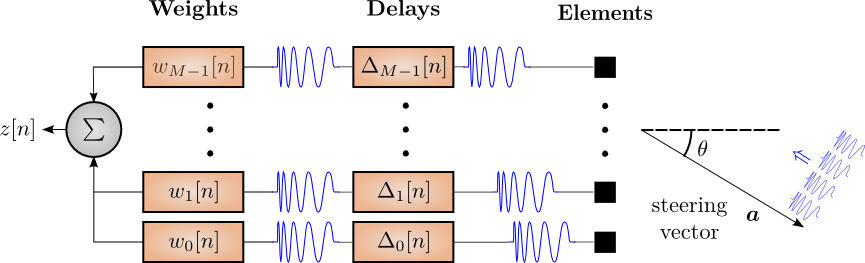
\includegraphics[width=3in]{gfx/beamforming_mv_lowres.png}
%\caption{}
%\label{fig:mv}
%\end{figure}

%Building and calculating the inverse of $\hat{R}$ is computational demanding, limiting the methods accessibility. Following the innovation in GPU computing, this has now started to change. 
%In this paper we introduce the first GPU implementation of the Capon beamformer capable of processing a 70 degree sector cardiac image from a 64 element phased array at interactive frame rates using both spatial and temporal smoothing. Both types of smoothing are important for maintaining delay-and-sum-like speckle and at the same time keep the high resolution property. This is achieved using complex base band data, which reduces the size of each range line to a minimum. In addition, complex data results in complex weights; hence this is a correct implementation of Capon beamforming with all degrees of freedom preserved. For high channel count systems we propose two ways of reducing computational complexity while maintaining 

\subsection{Beamspace Processing}\label{bs-capon}
Nilsen and Hafizovic \cite{Nilsen2009} have proposed to apply beamspace processing to reduce the required computations of the Capon beamformer when applied to medical ultrasound imaging. Beamspace is an alternative representation of the per-element data, transformed into a fan of beams covering the sector illuminated by transmit beams. The transformation is formally stated as
\begin{align}
\vec{x}_\text{BS}[n] &= \mat{B}\vec{x}[n], \ \ \ \ \ \ \ \ \ \ \ \ \ \, \mat{B} \in \mathbb{C}^{N,M} \label{eq:butler} \\ 
[\mat{B}]_{p,q} &= \frac{1}{\sqrt{M}}e^{-j 2 \pi p q / M} \ \ \ N \le M.
\end{align} 
The steering vectors in $\mat{B}$, the so-called Butler or normalized discrete fourier transform (DFT) matrix, determine each beam's direction in space. Beams where no interference is present can therefore be removed by simply removing rows from $\mat{B}$. 

For an imaging system using narrow transmit and receive beams, like cardiac ultrasound imaging, the received signal will be concentrated in a narrow band in wavenumber space. Hence, a small percentage of the beams will contain almost all the received energy. Nilsen and Hafizovic concluded that as little as three beams around (and including) the transmit direction were adequate to produce results comparable to applying Capon beamforming in element space. Hence, for equally pitched arrays the inversion steps is found to be constant with respect to the number of array elements.

The beamspace version of the Capon beamformer is derived by replacing the covariance matrix in (\ref{eq:w}) with the beamspace covariance matrix 
\begin{align}
\mat{\hat{R}}_\text{BS} = f(\vec{x}_\text{BS}) = f(\mat{B}\vec{x}), 
\end{align}
where $\mat{B} \in \mathbb{C}^{N_b,L}$, $N_b$ is the number of selected beams, and $f(\cdot)$ represent the covariance estimation process as defined in (\ref{eq:diag}).

In the remaining sections, the methods described in this section and Section \ref{sec:es-capon} will be referred to as beamspace Capon (BS-Capon) and element-space Capon (ES-Capon) respectively. The name Capon will refer to both methods. 

\subsection{GPU Compute Model}

%\textbf{(Ta med mer banale ting, dette er GPU for ultralydfolk)}

%\textbf{(Etter denne så må de forstå GPU og hvorfor MV passer.)}

In this section we give a brief discussion of GPU computing, laying the basis for our discussions on parallel implementation strategies. The Capon beamformers have been implemented using the CUDA GPU framework by Nvidia \cite{Nvidia2013}, however the challenges and proposed methods described in this paper are valid for other GPU framworks as well, like e.g. OpenCL. Independent of framework, the key point is that GPUs are designed to execute large sets of small concurrent tasks, like beamforming a pixel in a large image, much faster than a CPU. While the CPU has few cores, but logic to process complex threads, the GPU has many cores, but each core needs many (preferably simple) threads to keep it occupied and by that achieve maximum throughput.

In CUDA programming a kernel function is executed over a large set of threads, where the kernel function describes the work to be done in each thread. As depicted in Fig.\ \ref{fig:gpulayout}, threads are organized in a grid of thread-blocks, with maximal size of 1024 threads per block (e.g. $32\times32$). Threads inside a block support low-cost synchronization if needed. From a CUDA perspective the GPU consist of one or more streaming multi-processors (SM), where each SM is capable of executing multiple arithmetic operations per clock cycle.
%32 or more concurrent multiplications or additions, or both, depending on the architecture. A group of blocks is scheduled to each SM until all blocks have been processed.

An SM has a limited amount of shared memory (or near-core cache) and registers. Therefore, to achieve maximum GPU occupancy (defined as having the maximum number of threads residing on each SM), a conservative use of registers and shared memory per thread is required. Each thread should perform enough instructions per transferred byte in order to hide memory latency, and the problem should be divided into enough threads in order to hide instruction latency. Global GPU memory transactions, in addition to CPU-GPU transfers, are slow and must be minimized. All of these constraints combined pose a real challenge as the target problem has to map well to the GPU framework on both a grid, block, thread, and memory consumption level in order to benefit from parallel acceleration. In the next two sections, we will describe how this mapping can be done for the Capon beamformers.    

\begin{figure}
\centerline{\includegraphics[width=3.5in]{gfx/gpu_layout_vertical_2.eps}}
\caption{Calculation of Capon adaptive weights mapped to GPU architecture. A recorded echo across the array for a given range and angle (selected cell) is assigned to a group of $L$ threads that can run independently of all other groups. Note that several samples can be processed per thread-block if $L$ is small. The task of these $L$ threads is to calculate the Capon beamformer output in the three depicted steps.}
\label{fig:gpulayout}
\end{figure}

%When implementing algorithms on the GPU it is important to keep data as close to the core as possible. Utilizing available registers and shared memory to its maximum is therefore important.  

%More important, the CUDA 2.x compute capability (CC) has available 48 KB of near-core shared memory per SM that can be utilized by resident blocks. The maximum number of resident blocks per SM is 8, but in addition the maximum number of resident warps per SM is restricted to 48. Hence, with a block size of 512 only $48/(512/32) = 3$ blocks can occupy the SM at once. In addition, if one thread where to use 64B of shared memory the number of allowed resident blocks with a block size of 512 would be reduced to 1. Up to a curtain point it is beneficial to have as many warps as possible occupying the SM at once to hide latency from accessing memory. The SM has for CC 2.x 32K 32-bit long registers. When implementing algorithms on the GPU it is important to keep data as close to the core as possible. Utilizing available registers and shared memory to its maximum is therefore important.  

%\subsection{Optimizing kernel launch}
%Set the size of grid adaptively based on $L$, $M$ and $Yavg$.
%It is better to slide in space than time. $K$ is typically much larger than $2*Yavg + 1$.

% needed in second column of first page if using \IEEEpubid
%\IEEEpubidadjcol

\section{Parallel ES-Capon}\label{sec:meth}
In this section we will give a brief summary of our parallel implementation of the ES-Capon beamformer as presented in \cite{asen2012} and \cite{Buskenes}. This implementation was our starting point when the BS-Capon beamformer was implemented.   

If the beamformer in (\ref{eq:z_mv}) is analyzed in combination with the matrix equation in (\ref{eq:b}) and the covariance estimation process in (\ref{eq:diag}), we see that the calculation of a set of Capon weights is independent across the outputs $z[n]$. As shown in Fig.\ \ref{fig:gpulayout}, a first level of granularity is therefore to divide the image into a grid, where the output in each cell can be calculated independently. Further, based on memory dependencies and to hold memory consumption per thread at a minimum, a group of threads should process one output in the final image. Continuing with the calculation of one weight vector, the algorithm can be broken down into three main steps that, to some extent, can be divided further into a set of parallel processes. That is, for each data vector $\vec{x}$ in the image:
\begin{align*}
%\begin{array}{l}
\text{1) } &\text{Calculate the sample covariance matrix } \mat{\hat{R}} \text{ as in } \text{(\ref{eq:diag})}.\\
\text{2) } &\text{Solve the linear system of equations as in (\ref{eq:b}}).\\ %\vec{b} =\mat{\hat{R}}^{-1}\vec{1}_L\\
\text{3) } &\text{Calculate } \vec{w} = \vec{b}/\vec{1}_{L}^H\vec{b} \text{ and the amplitude as in (\ref{eq:z_mv})}.
%\end{array}
\end{align*}
%\begin{enumerate}
%\item Calculate the sample covariance matrix $\mat{\hat{R}}$ as in (\ref{eq:R})
%\end{enumerate}
%\begin{enumerate}
%\item[2)] Solve the linear system of equations $\mat{\hat{R}}\vec{b} =\vec{ 1}$
%\end{enumerate}
%\begin{enumerate}
%\item[3)] Calculate $\vec{w} = \vec{b}/\vec{1}^H\vec{b}$ and the amplitude $\vec{w}^H\vec{x}$
%\end{enumerate}
The computational complexities of these three steps are $O(N_KN_LL^2)$, $O(L^3)$, and $O(L)$, respectively. As $M$ (and thereby $L$) increases, the first two steps quickly become unmanageable, and real-time performance in cardiac ultrasound imaging can only be achieved by exploring methods with reduced complexity.

%(The three steps have, for modularity, been implemented using three different kernels. Joining all kernels into one could possible lead to an increase in speed.)

%\begin{figure}
%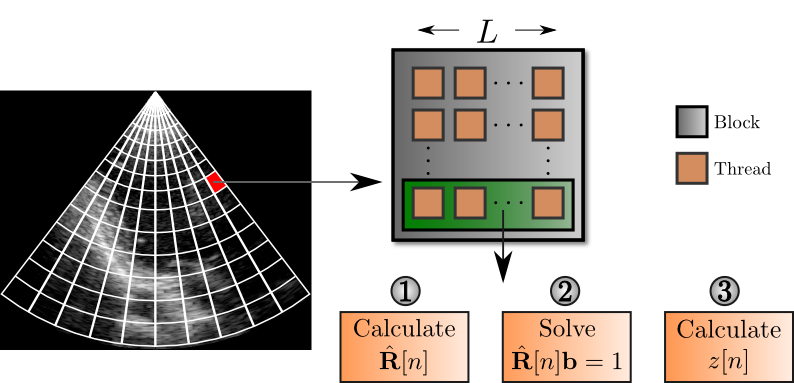
\includegraphics[width=3in]{gfx/gpu_layout_lowres.png}%
%\caption{}
%\label{fig:gpulayout}
%\end{figure}

\subsection{Calculation of Multiple Sample Covariance Matrices}\label{sec:calcR}

%The straightforward sum in (\ref{eq:R}) has complexity $O(L^2N_LN_K) = O(L^3)$ since $N_L$, the number of subarrays, is a function of $L$. This is actually the same as for inverting an $L \times L$ matrix. However little attention has been devoted to this step in the literature before. Note that for a typical array configuration we do more spacial smoothing than temporal smoothing. Hence, $N_K$ is usually small compared to $N_L$. The construction of $\mat{\hat{R}}$ is dominated by the number of elements $M$ ($N_L = M - L + 1$) for short subarrays, but since $L$ is selected in most cases to be between $M/2$ and $M/4$ a large $M$ implies a large $L$.

Calculation of one element of \R is from (\ref{eq:R}) found to be independent of calculation of the other elements. A natural level of granularity would then be to assign one thread to each element of $\mat{\hat{R}}$ \cite{Chen2011}. This will minimize global reads and writes needed per thread, but since we want to avoid block-to-block synchronization, the maximum supported subarray length is limited to 32 by this approach. Since most medical ultrasound arrays have 64 elements or more, an implementation not limited by $L_{max}=M/2=32$ is preferable.

In \cite{asen2012, Buskenes} we demonstrated how the cubic complexity with $L$ %and linear complexity with $N_K$ 
can be reduced by realizing that calculations in (\ref{eq:R}) overlap across subarrays. %Element $(i,j)$ of $\mat{\breve{R}}[n]$ can be calculated from element $(i-1, j-1), \text{for } i,j \in [1, L-1]$ in a sliding window maner as
%\begin{align}
%\mat{\breve{R}}_{i,j}[n] &=  \mat{\breve{R}}_{i-1,j-1}[n]  \nonumber \\
%&+ \sum_{n'=n-K}^{n+K} (x_{i+N_L-1}[n']x_{j+N_L-1}[n']^* \nonumber \\
%&- x_{i-1}[n']x_{j-1}[n']^H). \label{eq:sliding}
%\end{align}
%Along the time dimension we also find that
%\begin{align}
%\mat{\breve{R}}[n] &= \mat{\breve{R}}[n-1] + \sum_{l=0}^{N_L-1} (\vec{x}_l[n+K]\vec{x}_l[n+K]^H \nonumber \\
%&- \vec{x}[n-K-1]\vec{x}[n-K-1]^H).
%\end{align}
%- \mat{\breve{R}}[n-K-1] + \mat{\breve{R}}[n-K].
%Sliding windows across subarrays and in time can be realized simultaneously if $\mat{\hat{R}}$, averaged over subarrays, is calculated from an $N_K$-average in time of the outer products $\vec{x}[n]\vec{x}[n]^H$. However, since $N_K$ typically is small, and the GPU has a limited amount of shared memory available per thread, we focus on subarrays only. 
%In that case, 
The complexity of calculating $\mat{\hat{R}}$ is by this reduced to $O(N_K(L(N_L-2)+2L^2))$. For $L=M/2$ this reduces to $O(N_KM^2)$.
%The sliding-window approach will cause dependence among the iterative calculations. The level of task granularity is therefore increased. Calculations are still independent across time, but not along diagonals of $\mat{\hat{R}}$. One thread is therefore assigned to each diagonal in the upper triangle of $\mat{\hat{R}}$. For small values of $L$, several covariance matrices are calculated per thread block (Fig. \ref{fig:gpulayout}). 
Maximum supported $L$ is also increased to the maximum number of threads per block (currently 1024). %However, for small-$L$-high-$M$ configurations, memory consumption per thread will be too high to achieve full GPU occupancy.

%Taking symmetry into account, only the upper half of $\mat{\hat{R}}$ needs to be calculated. However, the GPU computes $\mat{\hat{R}}$ in such a way that the lower triangle can be found with little overhead \cite{Buskenes}. This also means that no special solver is needed in order to solve $\mat{\hat{R}}\vec{b} = \vec{1}_L$, even if a symmetric solver could have saved some instructions.

%For the adaptive diagonal loading factor in (\ref{eq:diag}), the trace of $\mat{\hat{R}}$ has to be known before diagonal elements are written back to global memory. One row for all covariance matrices is written to global memory per kernel iteration, the diagonal elements therefore need to reside in shared memory until the trace is accumulated. When that is done, scattered writes of the scaled diagonal elements to global memory has to be performed.

%For subarray averaging, the first row and column of $\mat{\hat{R}}$ has to be fully calculated, and for time averaging $\mat{\hat{R}}[0]$ has to be fully calculated.

%Since $L$ usually is larger than $N$, we have 

%Building $\hat{\mat{R}}$ using a sliding window approach across $K$ and $N_{avg}$. We have a limited amount of fast, near-core memory on the GPU. On NVIDIA architecture this memory is known as shared memory, and is restricted to 48KB per compute block. The maximum block size of 32x32, further restrict how large arrays we can handle inside a single compute block. It is therefore natural to restrict $L$ to a maxima of $32$ elements. Since $L \le M/2$, $M \le 64$. We can not afford to hold the full $\hat{\mat{R}}$ ($M = L$) when $\hat{\mat{R}} > 32$, because of limited amount of memory. ... Explain in detail how \texttt{buildR} is implemented in a kernel. ... Give more details on how much shared memory we have, and how it can be divided between compute blocks occupying one stream multiprocessor (SM).

%Discuss the bottleneck adaptive diagonal loading causes. Possible solutions includes, use trace from previous image, use pre-calculated array power, constant weight.

%Time averaging takes a lot of resources. It has been shown that time averaging can maintain both resolution and delay-and-sum-like speckle. The same speckle statistics can be obtain with small subarrays, but then we loose resolution. Small sub-arrays benefits from being less computational demanding.   

%\subsubsection{CUDA Compute Model}
%The CUDA compute model is based on execution of a kernel across a grid of compute threads. Each position in the grid holds a block of threads. Each block is further divided into groups of 32 threads, known as a warp. The maximum number of threads inside a block is restricted to 512, hence 16 warps. From a CUDA perspective the GPU consist of one or more stream multi processors (SM), %where each SM is capable of 32 or more, depending on the architecture, concurrent multiplications and/or additions. The CUDA 2.x compute capability (CC) has available 48 KB of near-core shared memory per SM that can be utilized by resident blocks. The maximum number of resident blocks per SM is 8, but in addition the maximum number of resident warps per SM is restricted to 48. Hence, %with a block size of 512 only $48/(512/32) = 3$ blocks can occupy the SM at once. In addition, if one thread where to use 64B of shared memory the number of allowed resident blocks with a block size of 512 would be reduced to 1. Up to a curtain point 
%it is beneficial to have as many warps as possible occupying the SM at once to hide latency from accessing memory and executing time consuming mathematical functions. The SM has for CC 2.x 32K 32-bit long registers. When implementing algorithms on the GPU it is important to keep data as close to the core as possible. Utilizing available registers and shared memory to its maximum is %therefore important.   

\subsection{Solving Multiple Small Linear Systems}
%The literature has mostly focused on large systems when solving systems of linear equations on the GPU. GPU libraries therefore often lack a comprehensive collection of batched solvers for large sets of small systems. The reason for this is two-fold. First the GPU needs to solve thousands of small systems in order to beat the low memory latency of the CPU. Second there is a range of system dimensions that does not fit well with the GPU architecture, where only a small amount of shared memory and registers are available. Because of this, it has been proven hard to optimize a manageable set of solvers that provides speedups compared to the CPU in every case. 

In \cite{asen2012} we discussed how it is not given that solving on the GPU is faster than solving on the CPU in general. However, there are two arguments for solving on the GPU. First the CPU, which might already run a lot of ultrasound-related algorithms, is offloaded. Second, the transfer of several thousand covariance matrices over the PCI-Express bus, from the CPU to the GPU, is avoided.

For the results presented in this paper, we have used a GPU implementation of batched Gauss-Jordan elimination made by Nvidia to solve $\mat{\hat{R}}\vec{b} = \vec{1}_L$, where $\vec{b} = \mat{\hat{R}}^{-1}\vec{1}_L$, for all pixels in an image in one kernel launch. The solver is available online for registered CUDA developers \cite{Nvidiaa}.%For smaller systems, $L < 10$, a direct solver using one thread per system is preferable. For this purpose we have implemented Cramer's rule for $2 \times 2$, $3 \times 3$ and $4 \times 4$ matrices. All solvers have been benchmarked against the latest Intel MKL libraries.

%However we will go through an implementation of an $\mat{U}^H\mat{D}\mat{U}$-decomposition-based solver to point out challenges when implementing batched solving of small linear systems on the GPU. ... (Unsure if this should be included).

%Can include details on GPU implementation of $\mat{U}^H\mat{D}\mat{U}$, but this has not proved to be faster than NVIDIA's GJ implementation. However, the complexity for solving with $\mat{U}^H\mat{D}\mat{U}$ decomposition is supposed to be $1/2$ of GJ.

%Skriv om utfordringene om å lage en solver på GPU. Ikke dra inn UHDU.

%In the final journal article we could discuss Conjugated gradient and Woodbury and the benefits they bring.
%Other solvers that provides different benefits includes Conjugated gradient and the use of the Woodbury matrix identity. 

\subsection{Compute Beamformer Output}
%The calculation of the beamformer output in (\ref{eq:z_mv}) has been implemented using one thread per element weight ($L$ threads per weight vector). After the solution vector $\vec{b}$ has been placed in shared memory, one of the $L$ threads finds the sum of $\vec{b}$. 
%Another option is to let several threads cooperate to form the sum using a binary reduction sum. However, in the following benchmarks the first approach has been used. 
%Each of the $L$ threads then reads one element of $\vec{b}$, and scales it with the inverse sum to get the weight vector $\vec{w}[n]$. 
The final output can be formed by either reducing the data down to length $L$ as in (\ref{eq:z_mv}), or increasing the weight vector to length $M$ as in (\ref{eq:z_mv2}). Since we selected to use $L$ threads per output, the data is reduced to length $L$ by letting thread $r$ calculate 
\begin{align}\label{eq:subsum}
\breve{x}_{r} = \sum_{k=r}^{r+N_L-1}x_{k} \text{ for } r \in [0, L-1].
\end{align}
Each thread now computes $z_r = w_r^*x_r$, and finally one thread computes and outputs $z = \frac{1}{N_L}\sum_{r=0}^{L-1} z_r$ to global memory. %The last sum can also be performed using a binary reduction sum across several threads for increased speed.


\begin{figure}
\centerline{\includegraphics[width=3.2in]{gfx/gpu_layout_bs_2.eps}}
\caption{Calculation of the sliding beamspace transform. A group of $N_b$ threads is assigned a set of subarrays which they transform to beamspace in a sliding window fashion. In this example $N_b=3$, $l$ is the current subarray and $k$ is the current beam.}
\label{fig:gpulayoutbs}
\end{figure}

\section{Parallel BS-Capon}\label{sec:bs}
In this section we will derive a parallel implementation of the BS-Capon beamformer, and comment on how it deviates from the implementation in Section \ref{sec:meth}. The three main steps described in Section \ref{sec:meth} are present here as well, but in addition we need to transform the per-element data to beamspace. This can be done using a FFT, but for few beams ($N_b < \log{L}$) a matrix multiply with the truncated Butler matrix is less costly. 

In order to reduce the complexity of the matrix inversion problem the transformation must be performed before or after the covariance matrix has been estimated. If the transformation is applied before, one transformation is needed per subarray. This results in subarrays that no longer overlap. The amount of input data are therefore changed from $M$ to $N_LN_b$ elements per sample, but all remaining steps should get lower computational complexity as long as $N_b < L$.

The other option is to transform the element space covariance matrix to beamspace:
\begin{align}
\mat{\hat{R}}_\text{BS} &= \mat{B}\mat{\hat{R}}\mat{B}^H.
\end{align}
The advantage of this approach is that minor changes have to be made to the pipeline described in Section \ref{sec:meth}, but it will only speed up the solving step if the solution $\vec{b}_{BS}$ is transformed back to element space. In this paper we will focus on the first approach, and how it has been implemented on the GPU.
%By this approach we go from solving $\mat{\hat{R}}\vec{b} = \vec{1}_L$, which is an $L \times L$ system, to solving the $N_b \times N_b$ system $\mat{\hat{R}}_{BS}\vec{b}_{BS} = (\sqrt{L}\vec{e}_1)$. Now, one can either choose to transform the subarray sums, as in (\ref{eq:subsum}), to beamspace or transform the result, $\vec{b}_{BS}$, back to element space. 
In both cases solving has to be performed against a beamspace steering vector
\begin{align}
\vec{a}_\text{BS} &= \mat{B}\vec{1}_L = \sqrt{L}\vec{e}_1,
\end{align}
where $\vec{e}_i$ has the value one in the $i$th position and zeroes elsewhere. Note that the factor $\sqrt{L}$ was not included in \cite{Nilsen2009}.

As mentioned, transforming subarrays into beamspace yields subarrays that no longer overlap. This means that the spatial overlap previously exploited when calculating the sample covariance matrix in element space is no longer available. On the other hand, since $N_b$ should be small ($N_b < 32$), one thread assigned to each element in $\mat{\hat{R}}_\text{BS}$ is now an option. A kernel similar to the one described in \cite{Chen2011} has therefore been implemented. The computational complexity of this step is now $O(N_KN_LN_b^2)$, which for $L=M/2$ is less than the complexity of building $\mat{\hat{R}}$ in element space as long as $N_b < \sqrt{M}$.

%The implementation calculating covariance matrices therefore needs to be adjusted to handle non-overlapping subarrays. The complexity of constructing the covariance matrix is changed to $O(N_b^2L)$, so constructing the covariance matrices will be faster in beamspace as long as $N_b < \sqrt{L}$.
%Derivation of sliding beamspace transformation. 
%We will now show how to minimize the amount of operations required for the beamspace transformation by utilizing the overlap between subarrays previously exploited when estimating the covariance matrix in element space. 
The overlap between subarrays that were exploited when estimating the covariance matrix in element space, can now be utilized when calculating the beamspace transform. 
Given a $M$ long data vector divided into $N_L$ subarrays, the beamspace transformation of the $l$th subarray for the $k$th beam is from (\ref{eq:butler}) found to be:
\begin{align}\label{eq:bs_formula}
x_{\text{BS},l,k} &= \mat{B}_k\vec{x}_l \,\,\,\,\,\,\,\,\, k \in [0, N_b-1] \\
&= \frac{1}{\sqrt{L}}\sum_{p=i}^{l+L-1}x_p e^{-j2\pi k(p-l)/L},
\end{align}
where $\mat{B}_k$ is the $k$th row of $\mat{B}$. %Manipulating this expression we find that for $l \in [1, L-1]$
%\begin{align}\label{eq:sliding_bs}
%x_{\text{BS},l,k} &= \frac{1}{\sqrt{L}}((x_{\text{BS},l-1,k} - x_{l-1})e^{-j2\pi k/L} \nonumber \\ &+ x_{i+L-1}e^{-j2\pi k(L-1)/L}) \nonumber \\
%&= \frac{1}{\sqrt{L}}(x_{\text{BS},l-1,k} - x_{l-1} + x_{i+L-1})e^{-j2\pi k/L}.
%\end{align}

%We denote this the sliding-window beamspace transformation (SBS), and it is equal to a normalized sliding DFT \cite{Lyons2003}. For $l=0$ a full computation has to be performed using (\ref{eq:bs_formula}).
This formula has been implemented using a normalized sliding DFT (SDFT)\cite{Lyons2003}.
%Equation (\ref{eq:sliding_bs}) shows that 
The SDFT allows us to still save instructions by utilizing the overlap between subarrays, but with an increase in task level granularity. In this situation, it might be tempting to use one thread per beam (index $k$) that calculates this beam for all subarrays. However, since the number of selected beams usually is small ($N_b \ll M$) we will end up with a large memory-per-thread ratio ($M/N_b$). Using one thread per beam is therefore not feasible for small-$N_b$-large-$M$ configurations. One solution, as depicted in Fig.\ \ref{fig:gpulayoutbs}, is to combine SDFT with full computations. A number of sub thread groups of size $N_b$ is created that targets different sets of subarrays which they transform using the SDFT algorithm. In that way, the number of threads per sample is increased and thus the memory-per-thread ratio is decreased. 

After solving $\vec{b}_\text{BS} = \sqrt{L}\mat{\hat{R}}_\text{BS}^{-1}\vec{e}_1$, the beamspace weight vector is calculated as 
\begin{align}
\vec{w}_\text{BS} = \frac{\vec{b}_\text{BS}}{\sqrt{L}\vec{e}_1\vec{b}_\text{BS}} \in \mathbb{C}^{N_b}
\end{align}  
using one thread per beam, and applied to the beamspace data summed across subarrays,
\begin{align}
z[n] = \vec{w}_\text{BS}^H\sum_{l=0}^{L-1}\vec{x}_{\text{BS},l}. 
\end{align}
%Several pixels are calculated per thread block for small values of $N_b$ in order to achieve high GPU occupancy. The beamspace data summed across subarrays are calculated as part of the SBS kernel.   

%How do we calculate the number of possible subarrays $N_L$ with overlap $L-s$ in a data vector of length $M$.
%\begin{align}
%N_L = floor(\frac{M}{s}) - floor(\frac{L-1}{s})
%\end{align}

As presented in (\ref{eq:diag}), adaptive diagonal loading is performed by loading the sample covariance matrix with the average energy per element, that is $\text{trace}\{\mat{\breve{R}}\}/L$. When data are transformed into beamspace, a high percentage of the total energy is mapped to a small subset of beams. Therefore, if a set of high energy beams is selected, the average energy per beam will be higher than the average energy per element ($\text{trace}\{\mat{\breve{R}}\}/L < \text{trace}\{\mat{\breve{R}}_{\text{BS}}\}/N_b$). This means that less diagonal loading (smaller $d$) has to be applied when the covariance is estimated among beams and not elements. 

To summarize, by transforming data to beamspace the complexity of all subsequent steps is potentially reduced. Calculation of the covariance matrix is now $O(N_KN_LN_b^2)$, the inversion step is $O(N_b^3)$, and calculation of weights and the beamformer output are both $O(N_b)$. The added complexity of SDFT is $O(N_bL)$. To maximize performance, large adjustments to the processing pipeline described in Section \ref{sec:meth} is required. 

%(Go in detail about the implementation using sliding DFT).

%(Go in detail about what kind of modifications we need to do to each of the three steps)

%Note that $\mat{B}\mat{B}^H = \mat{I}$ and $\mat{B}^H\mat{B} \ne \mat{I}$ when $N_b < L$.

%Another way of computing the beamspace transformation is to transform the steering vector $\vec{a}$ and covariance vector $\mat{\hat{R}}$ beforing solving the following system of linear equations: $(\mat{B}\mat{\hat{R}}\mat{B}^H)^{-1}(\mat{B}a) = b_{BS}$.

%\subsection{Iterative Capon}
%The idea behind iterative Capon is to perform Capon using small subarrays in several iterations until there is only two subarrays to sum. In this way we fix the size of L, hence the complexity of solving $\mat{R}\vec{b} = \vec{1}$. However, for each iteration we re-obtain L-1 degrees of freedom until all are retrieved after $K = M-L+1$ iterations. Since subarray averaging has been applied to decorrelated the signal, we might loose this effect when reestablishing all degrees of freedom. The number of iterations should therefore be restricted to $K/2$ to equal the normal choice of $L = M/2$ when it comes to degrees of freedom. 
 

\section{Benchmarks}\label{sec:bench}

%Describe the computer system (CPU, GPU...). Describe the data that are processed (field II, Channel data from GE Vingmed).
% stolpediagram, med de ulike metodenes kjøretid oppehverandre.

\begin{figure*}[!t]
\centerline{
\subfloat[]{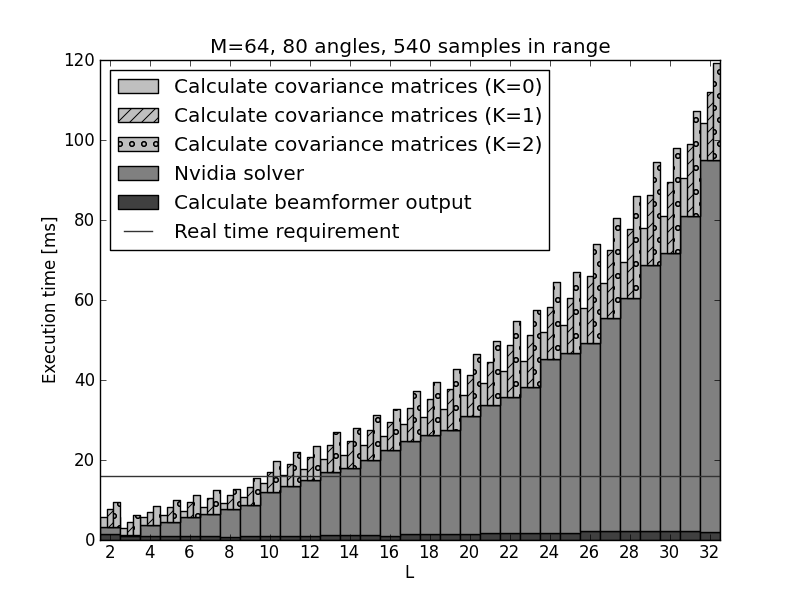
\includegraphics[width=3.4in]{gfx/benchmark_bar_64_80_540.png} \label{fig:benchUS64}}
\hfil
\subfloat[]{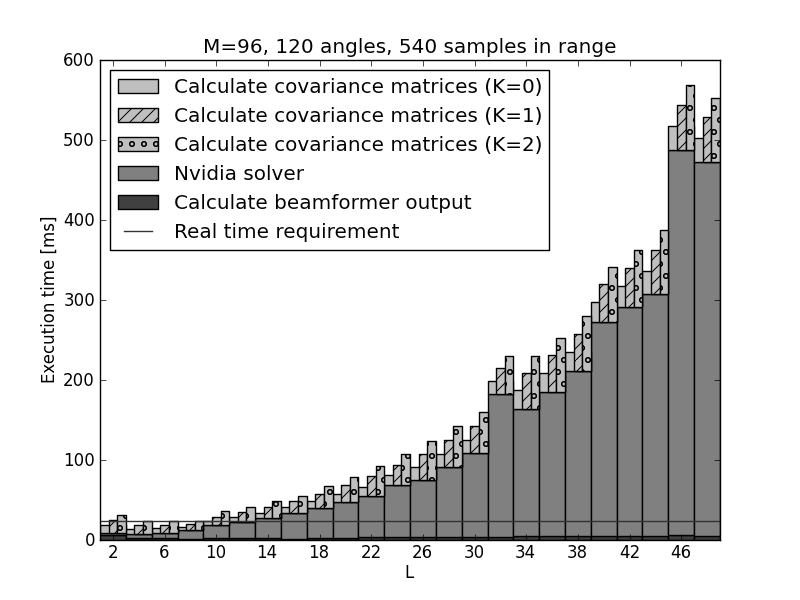
\includegraphics[width=3.4in]{gfx/benchmark_bar_96_120_540.png}%
\label{fig:benchUS96}}}
%\centerline{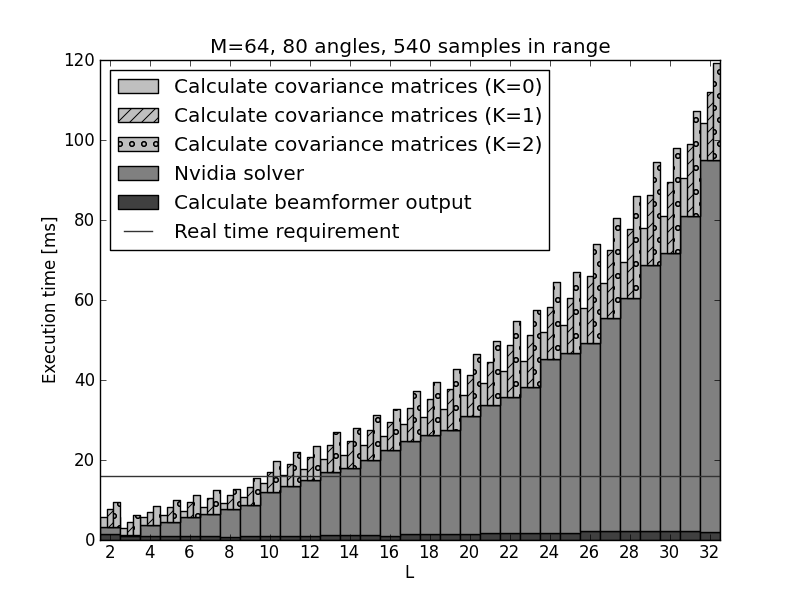
\includegraphics[width=3.5in]{gfx/benchmark_bar_64_80_540.png}}
\caption{Benchmarks of GPU Capon beamforming in element space for a cardiac image covering a $70\degree$ wide $15.4$ cm deep sector. Execution time is plotted as a function of subarray length $L$. The figures show execution times for the three steps listed in Section \ref{sec:meth}: Calculating covariance matrices with three different choices of temporal averaging, solver, and the final beamformer sum.}
\label{fig:bench}
\end{figure*}

\begin{figure*}[!t]
\centerline{\subfloat[]{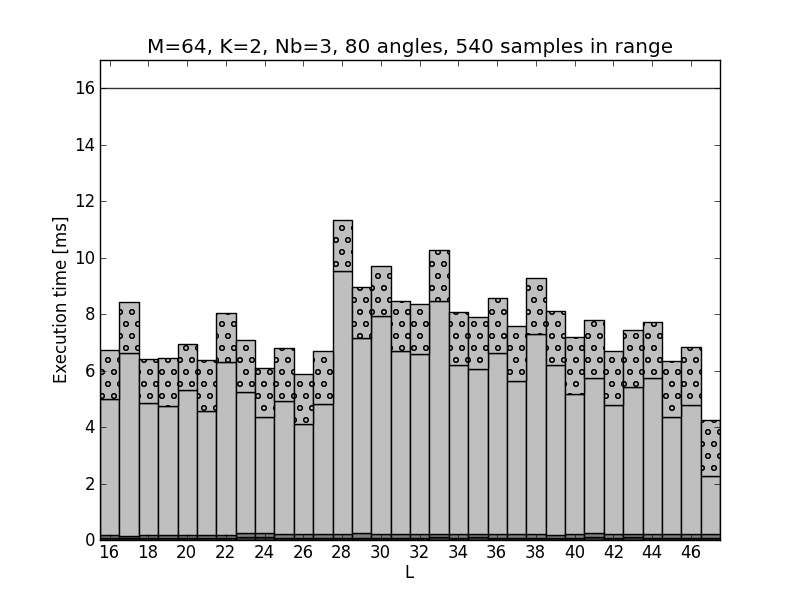
\includegraphics[width=3.4in]{gfx/benchmark_bar_bs_M=64_Nx=80_Ny=540_Nb=3.png} \label{fig:benchBS64}}
\hfil
\subfloat[]{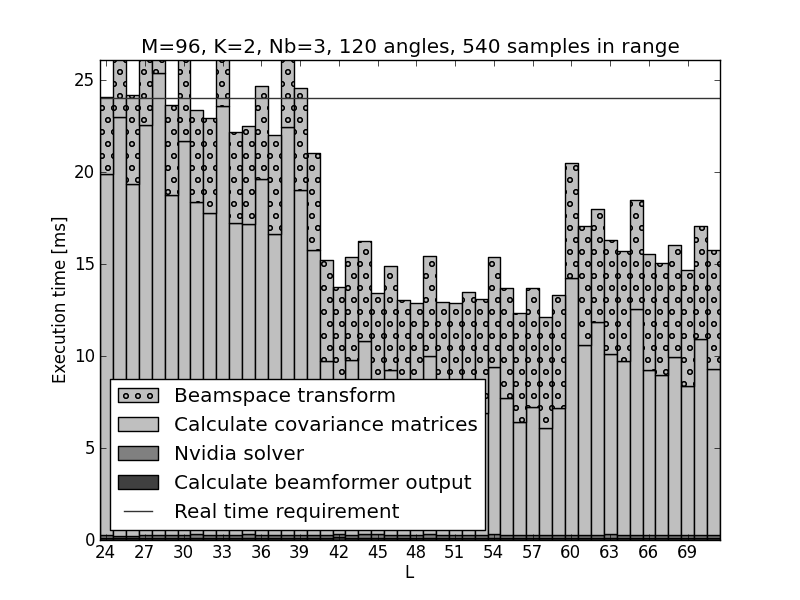
\includegraphics[width=3.4in]{gfx/benchmark_bar_bs_M=96_Nx=120_Ny=540_Nb=3.png}%
\label{fig:benchBS96}}}
\caption{Benchmarks of GPU beamspace Capon beamforming for a cardiac image covering a $70 \degree$ and $15.4$ cm deep sector. Execution time is plotted as a function of subarray length $L$.  If $L$ had been fixed at $M/2$ and execution time was plotted against $N_b$, the solver would have shown the same quadratic growth as in Fig.\ \ref{fig:bench}. When $N_b$ is fixed, calculating the covariance matrix and the BS-transform is inverse proportional and proportional to $L$ respectively. The large jumps in execution times are caused by adaptive kernel launch configurations, which depends on $M$, $L$ and $N_b$.}
\label{fig:benchBS}
\end{figure*}
In this section we present benchmarks of the implementations presented in Sections \ref{sec:meth} and \ref{sec:bs} performed on a Nvidia Quadro 6000 graphics card (14 SMs, 1 TFlops theoretical single precision performance, 6 GB global memory, and 144 GB/s memory bandwidth). Problem sizes are calculated based on 64 and 96 element phased arrays with a 3.4 MHz center frequency. Assuming a system bandwidth of 80\% (relative to the center frequency) we need a complex sampling frequency of 2.7 MHz, and when imaging down to a depth of 15.4 cm we have approximately 540 samples per range line. The angular sampling is given by the Rayleigh criterion divided by two \cite{Hergum2007}, 
\begin{equation}\label{eq:rayleigh}
\delta{}\theta = \lambda/(2Mp),
\end{equation}
where $\lambda$ is the pulse wavelength and $p$ is the element pitch. 
To sample a $70\degree$ sector with $64$- and $96$-element arrays with $p=\lambda/2$ we therefore need approximately 80 and 120 receive beams respectively. 

The presented execution times do not include transfer of data from CPU- to the GPU-side, since data are assumed to be pre-delayed and available in global GPU memory. This is a valid assumption, since the imaging scenarios presented in this paper are well below the 8.0 GB/s limit of PCI Express 2.0. What is included are all calculations, memory transfers from global to shared GPU memory, and shared memory access. The delay step has previously been shown to take far less time than what we report for both Capon beamformers \cite{Song2012, Chen2011}.

Benchmarks of the ES-Capon beamformer are presented in Fig.\ \ref{fig:bench}. For each subarray size, the total execution time is split into one bar for each of the three steps described in Section \ref{sec:meth}, and the calculation of $\mat{\hat{R}}$ is presented for three different values of $K$. For $M=64$, $L=32$ and $K=2$, a typical setup for high-quality cardiac imaging, processing throughput is 8.3 frames per second (FPS). For $M=96$, $L=48$ and $K=2$ the processing throughput drops below $0.5$ FPS.

In Fig.\ \ref{fig:benchBS} we present similar benchmarks for the BS-Capon beamformer. The figure only presents results with use of temporal averaging ($K=2$). For $M=64$, $L=32$, $K=2$ and $N_b=3$, processing throughput is 125 FPS (8 ms). For $M=96$, $L=48$, $K=2$ and $N_b=3$, processing throughput is 77 FPS (13 ms). In all four benchmarks there is a line indicating the time it takes to acquire the underlying image using one receive line per transmit. Hence, below this line we are capable of performing real-time processing.

\section{In-vivo cardiac images}\label{sec:images}

%\begin{figure*}[!t]
%\centerline{
%\subfloat[]{ 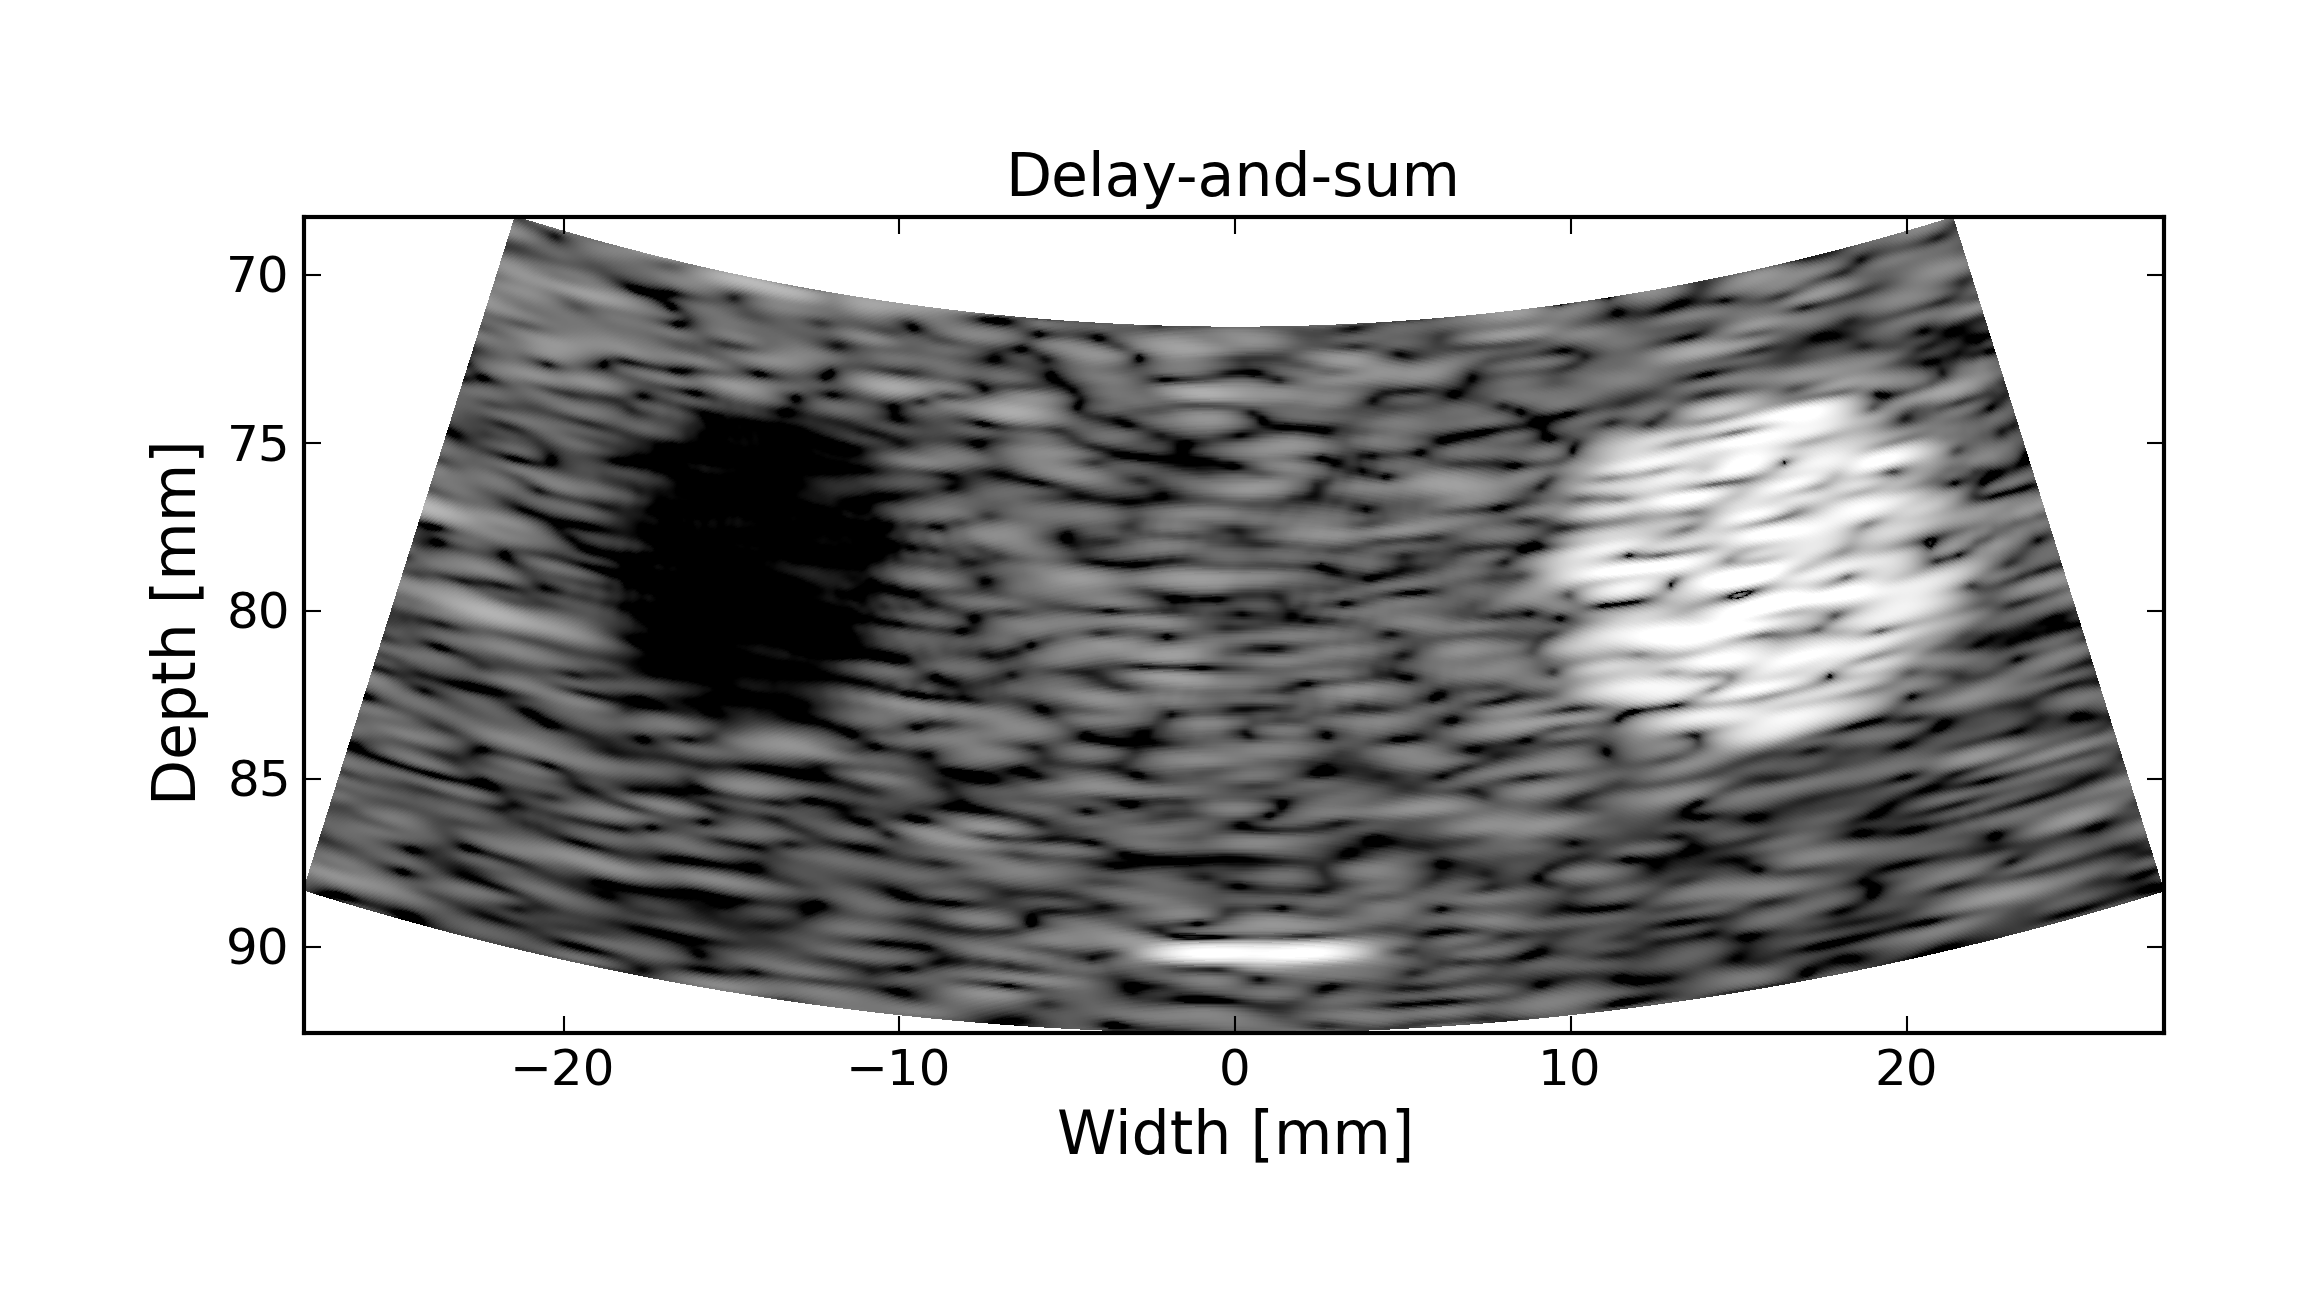
\includegraphics[width=2.2in]{gfx/das.png} \label{fig:phantomDAS} }
%\hfil
%\subfloat[]{ 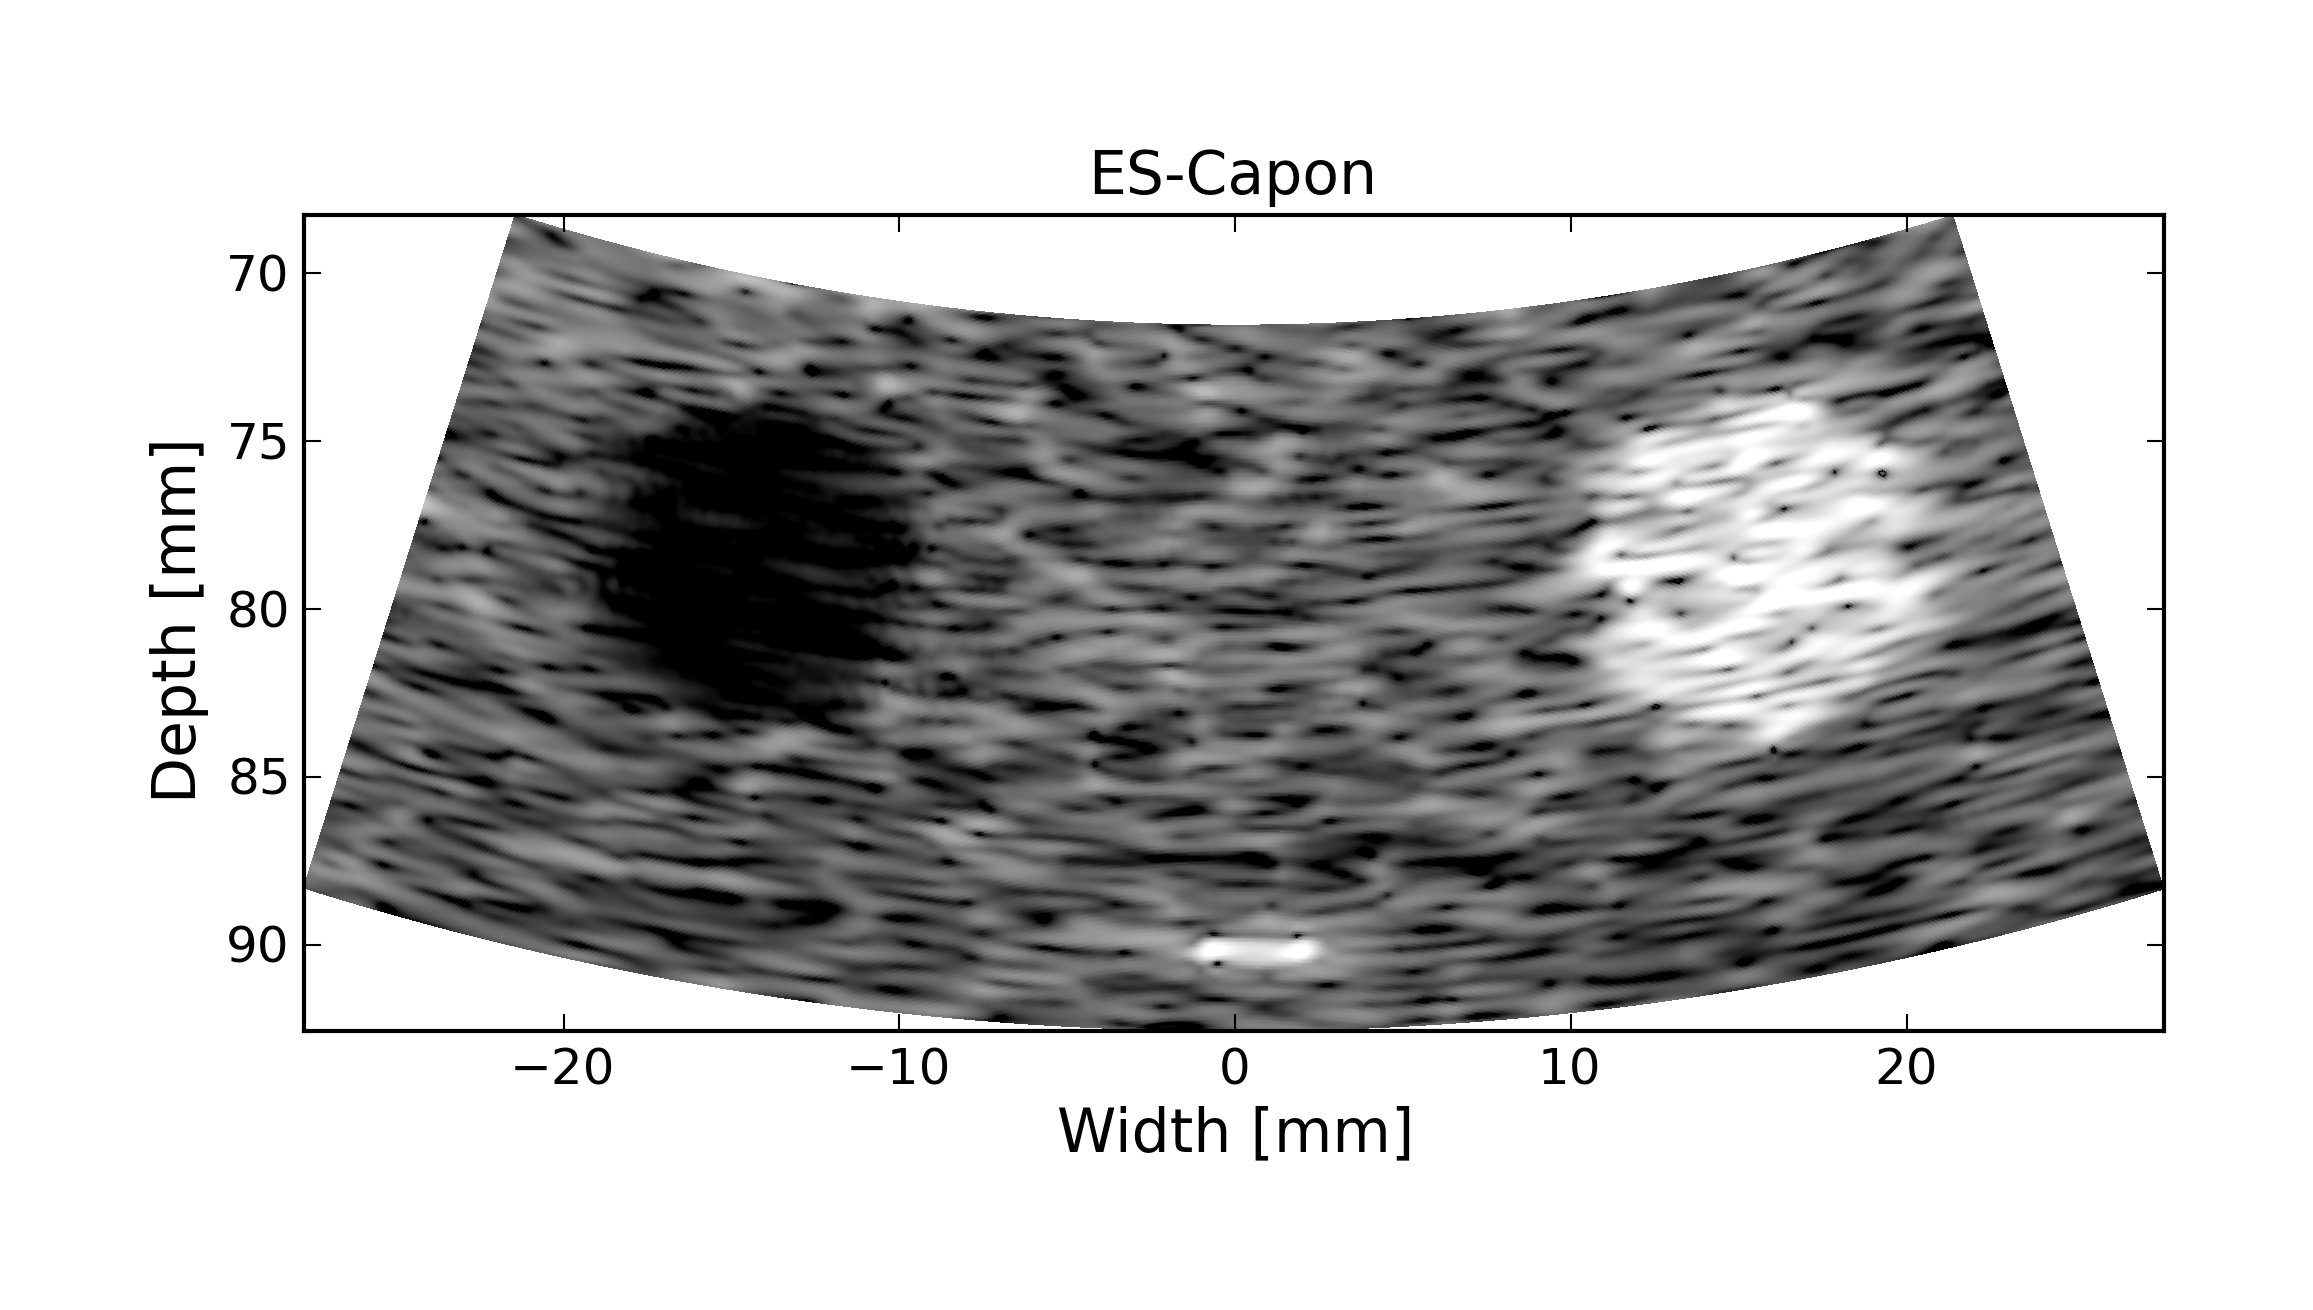
\includegraphics[width=2.2in]{gfx/capon.png} \label{fig:phantomMV} }
%\hfil
%\subfloat[]{ 
%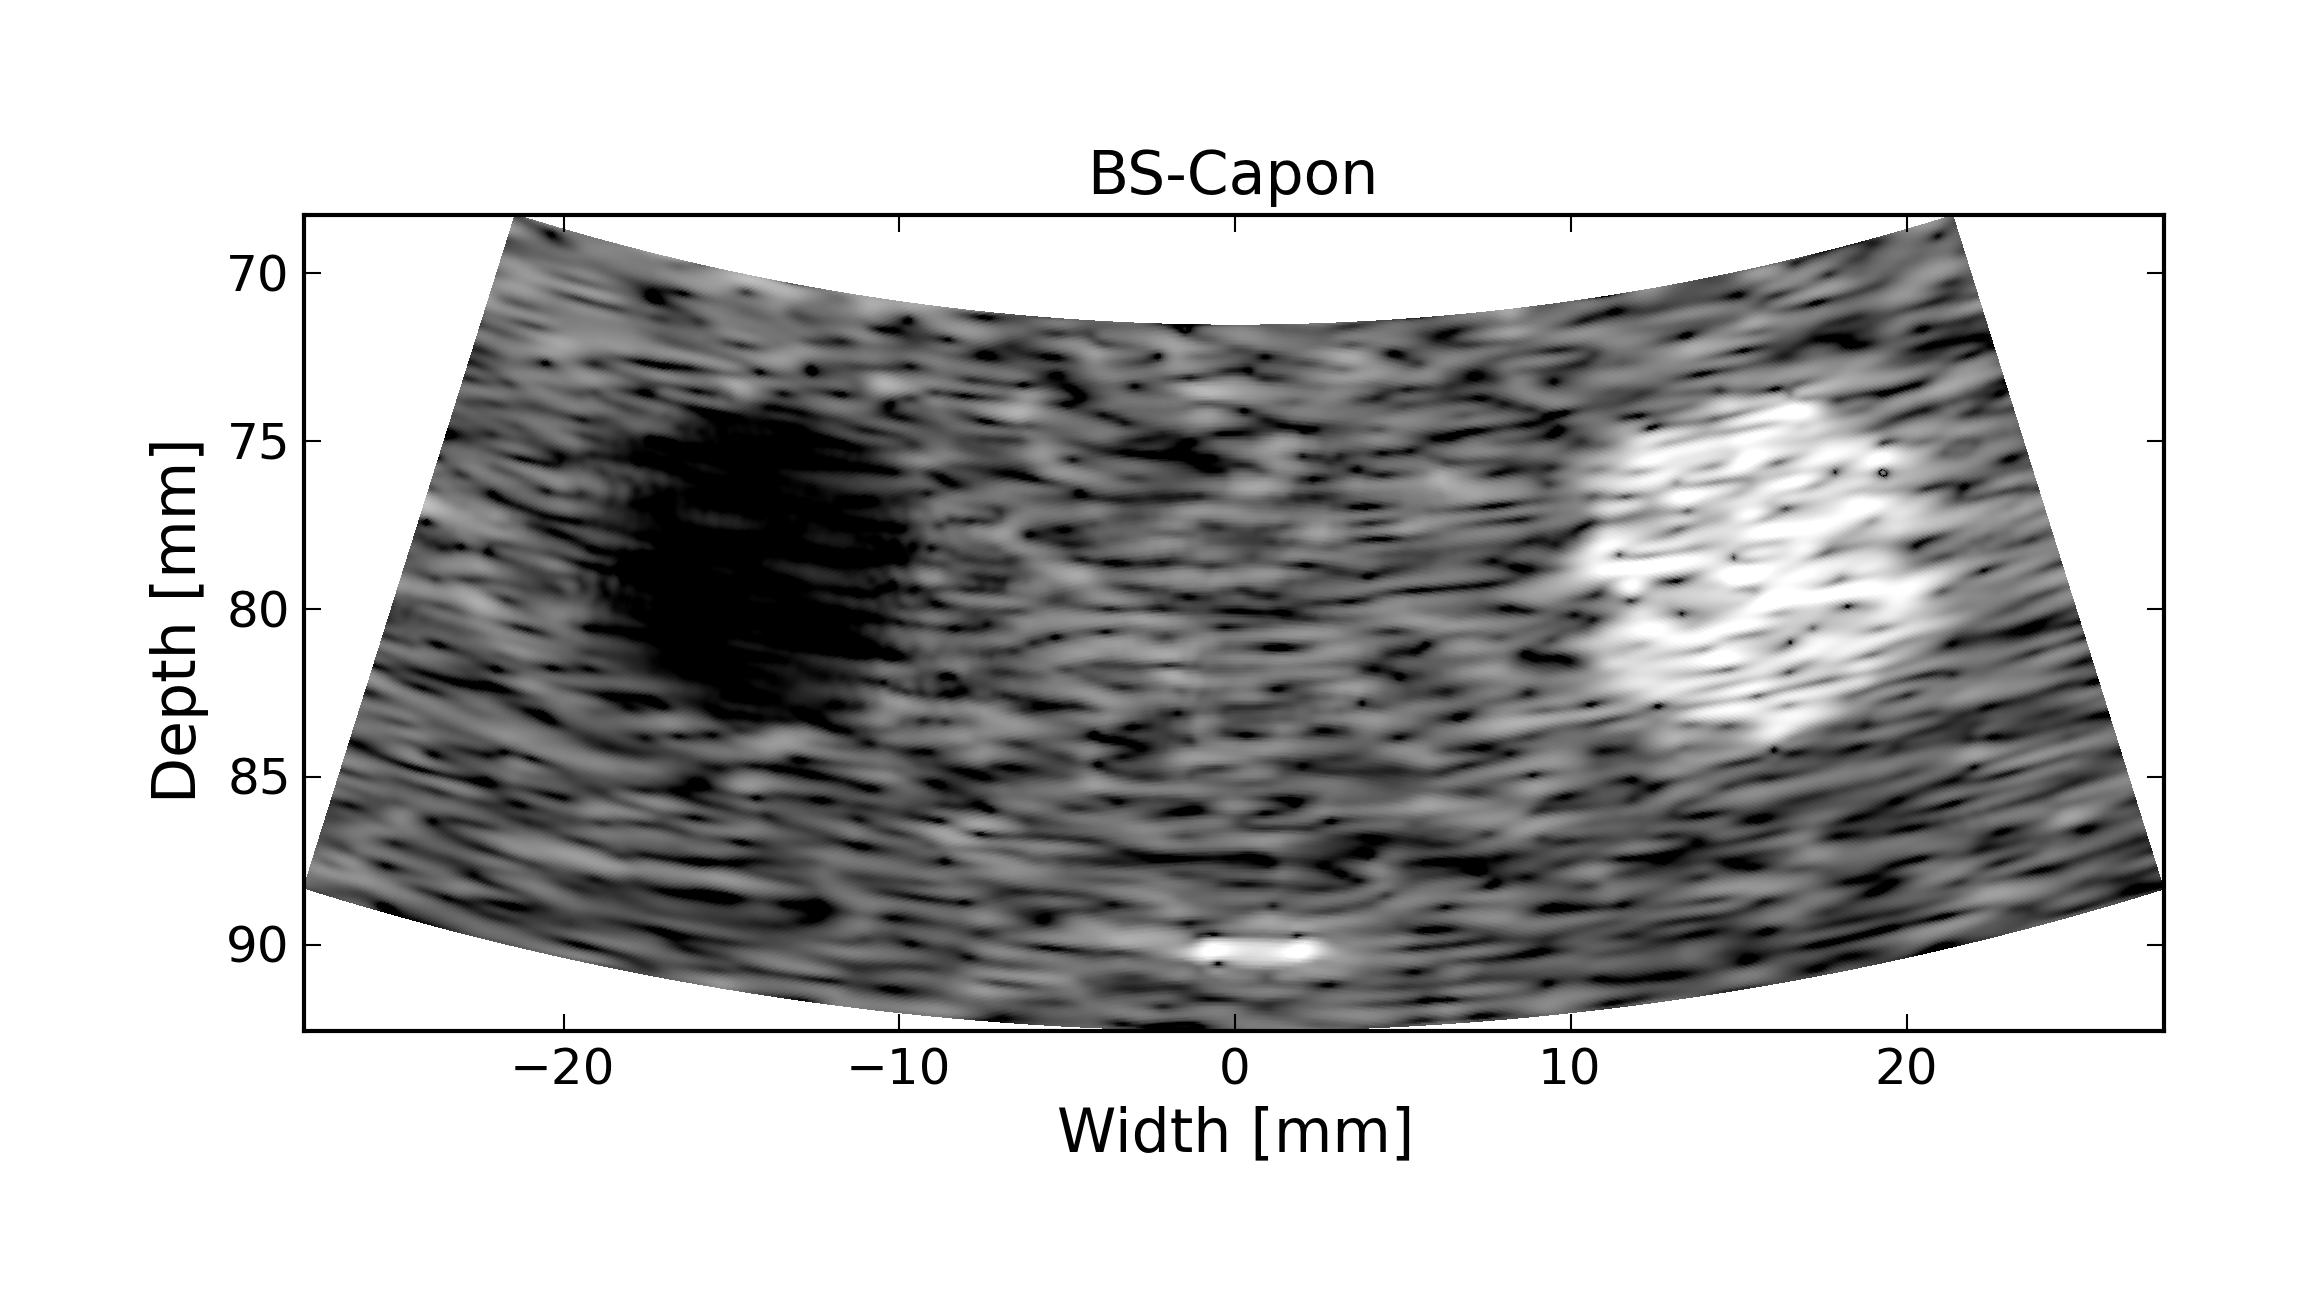
\includegraphics[width=2.2in]{gfx/capon_bs.png} \label{fig:phantomBS} 
%\hfil
%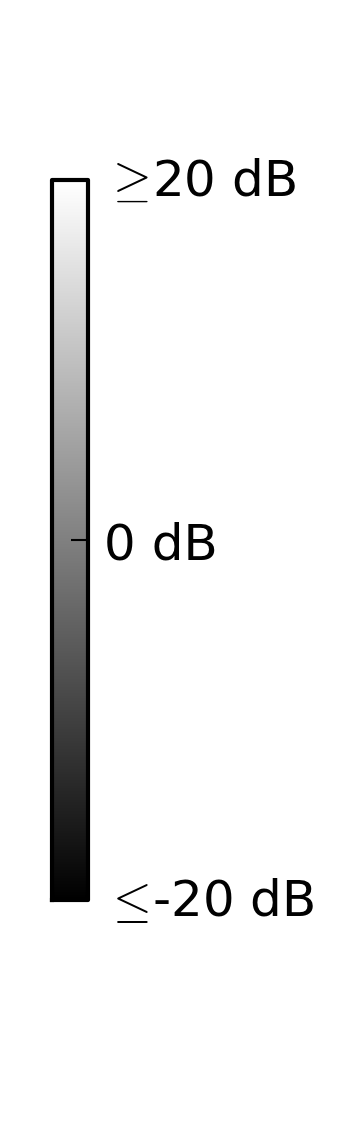
\includegraphics[width=0.35in]{gfx/colorBarPhantom2.png}
%}
%}
%\caption{Simulated phantom containing one bright (20 dB) and one dark (-20 dB) circular area and two point targets (30 dB) in speckle (0 dB). The simulation was done using Field II with a 64-element, 3.4 MHz, and $\lambda/2$ pitch phased array. Dynamic range is -20 dB to 20 dB with mean value represented as 0 dB. The image is the 15th frame in the attached videos. a) Delay-and-sum with uniform weights. b) Element-space Capon ($L=32, K=2, d=0.1$) \multimedia{Media-Movie 1}. c) Beamspace Capon ($L=32, K=2, N_b=3, d=0.01$) \multimedia{Media-Movie 2}.}
%\label{fig:phantom}
%\end{figure*}

\begin{figure*}[!t]
\centerline{
\subfloat[]{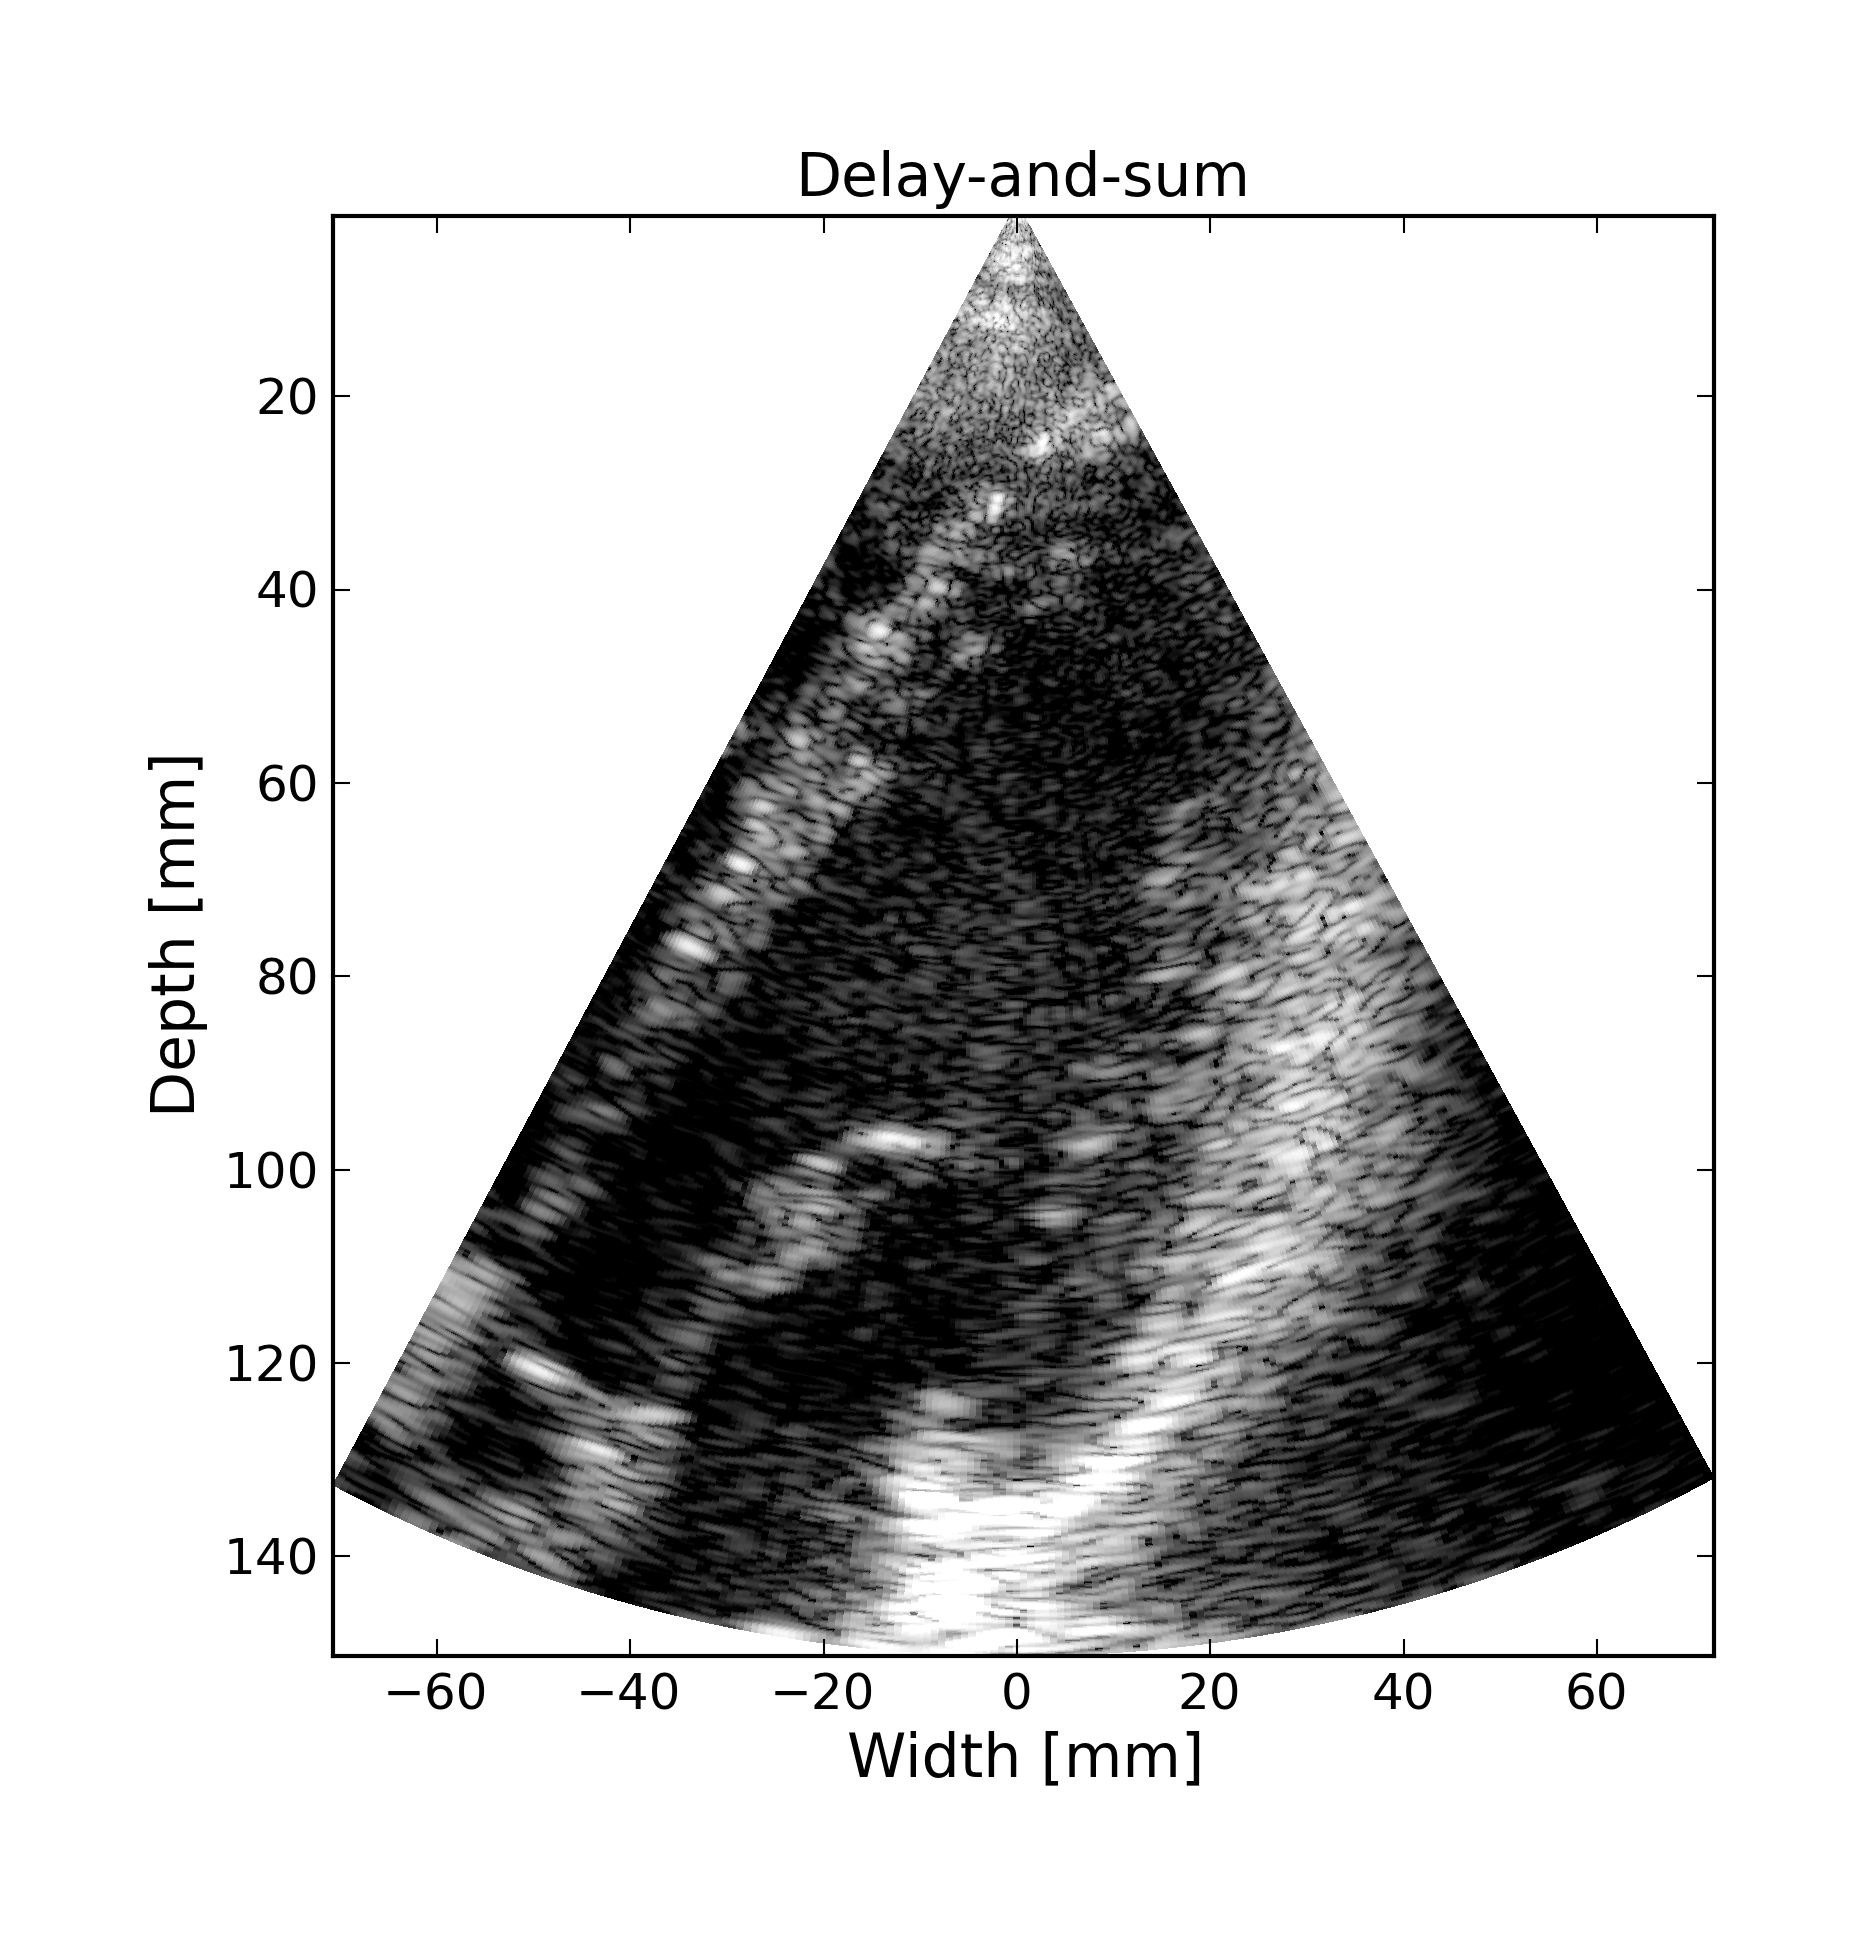
\includegraphics[width=2.2in]{gfx/das_invivo.png} \label{fig:invivoDAS}}
\hfil
\subfloat[]{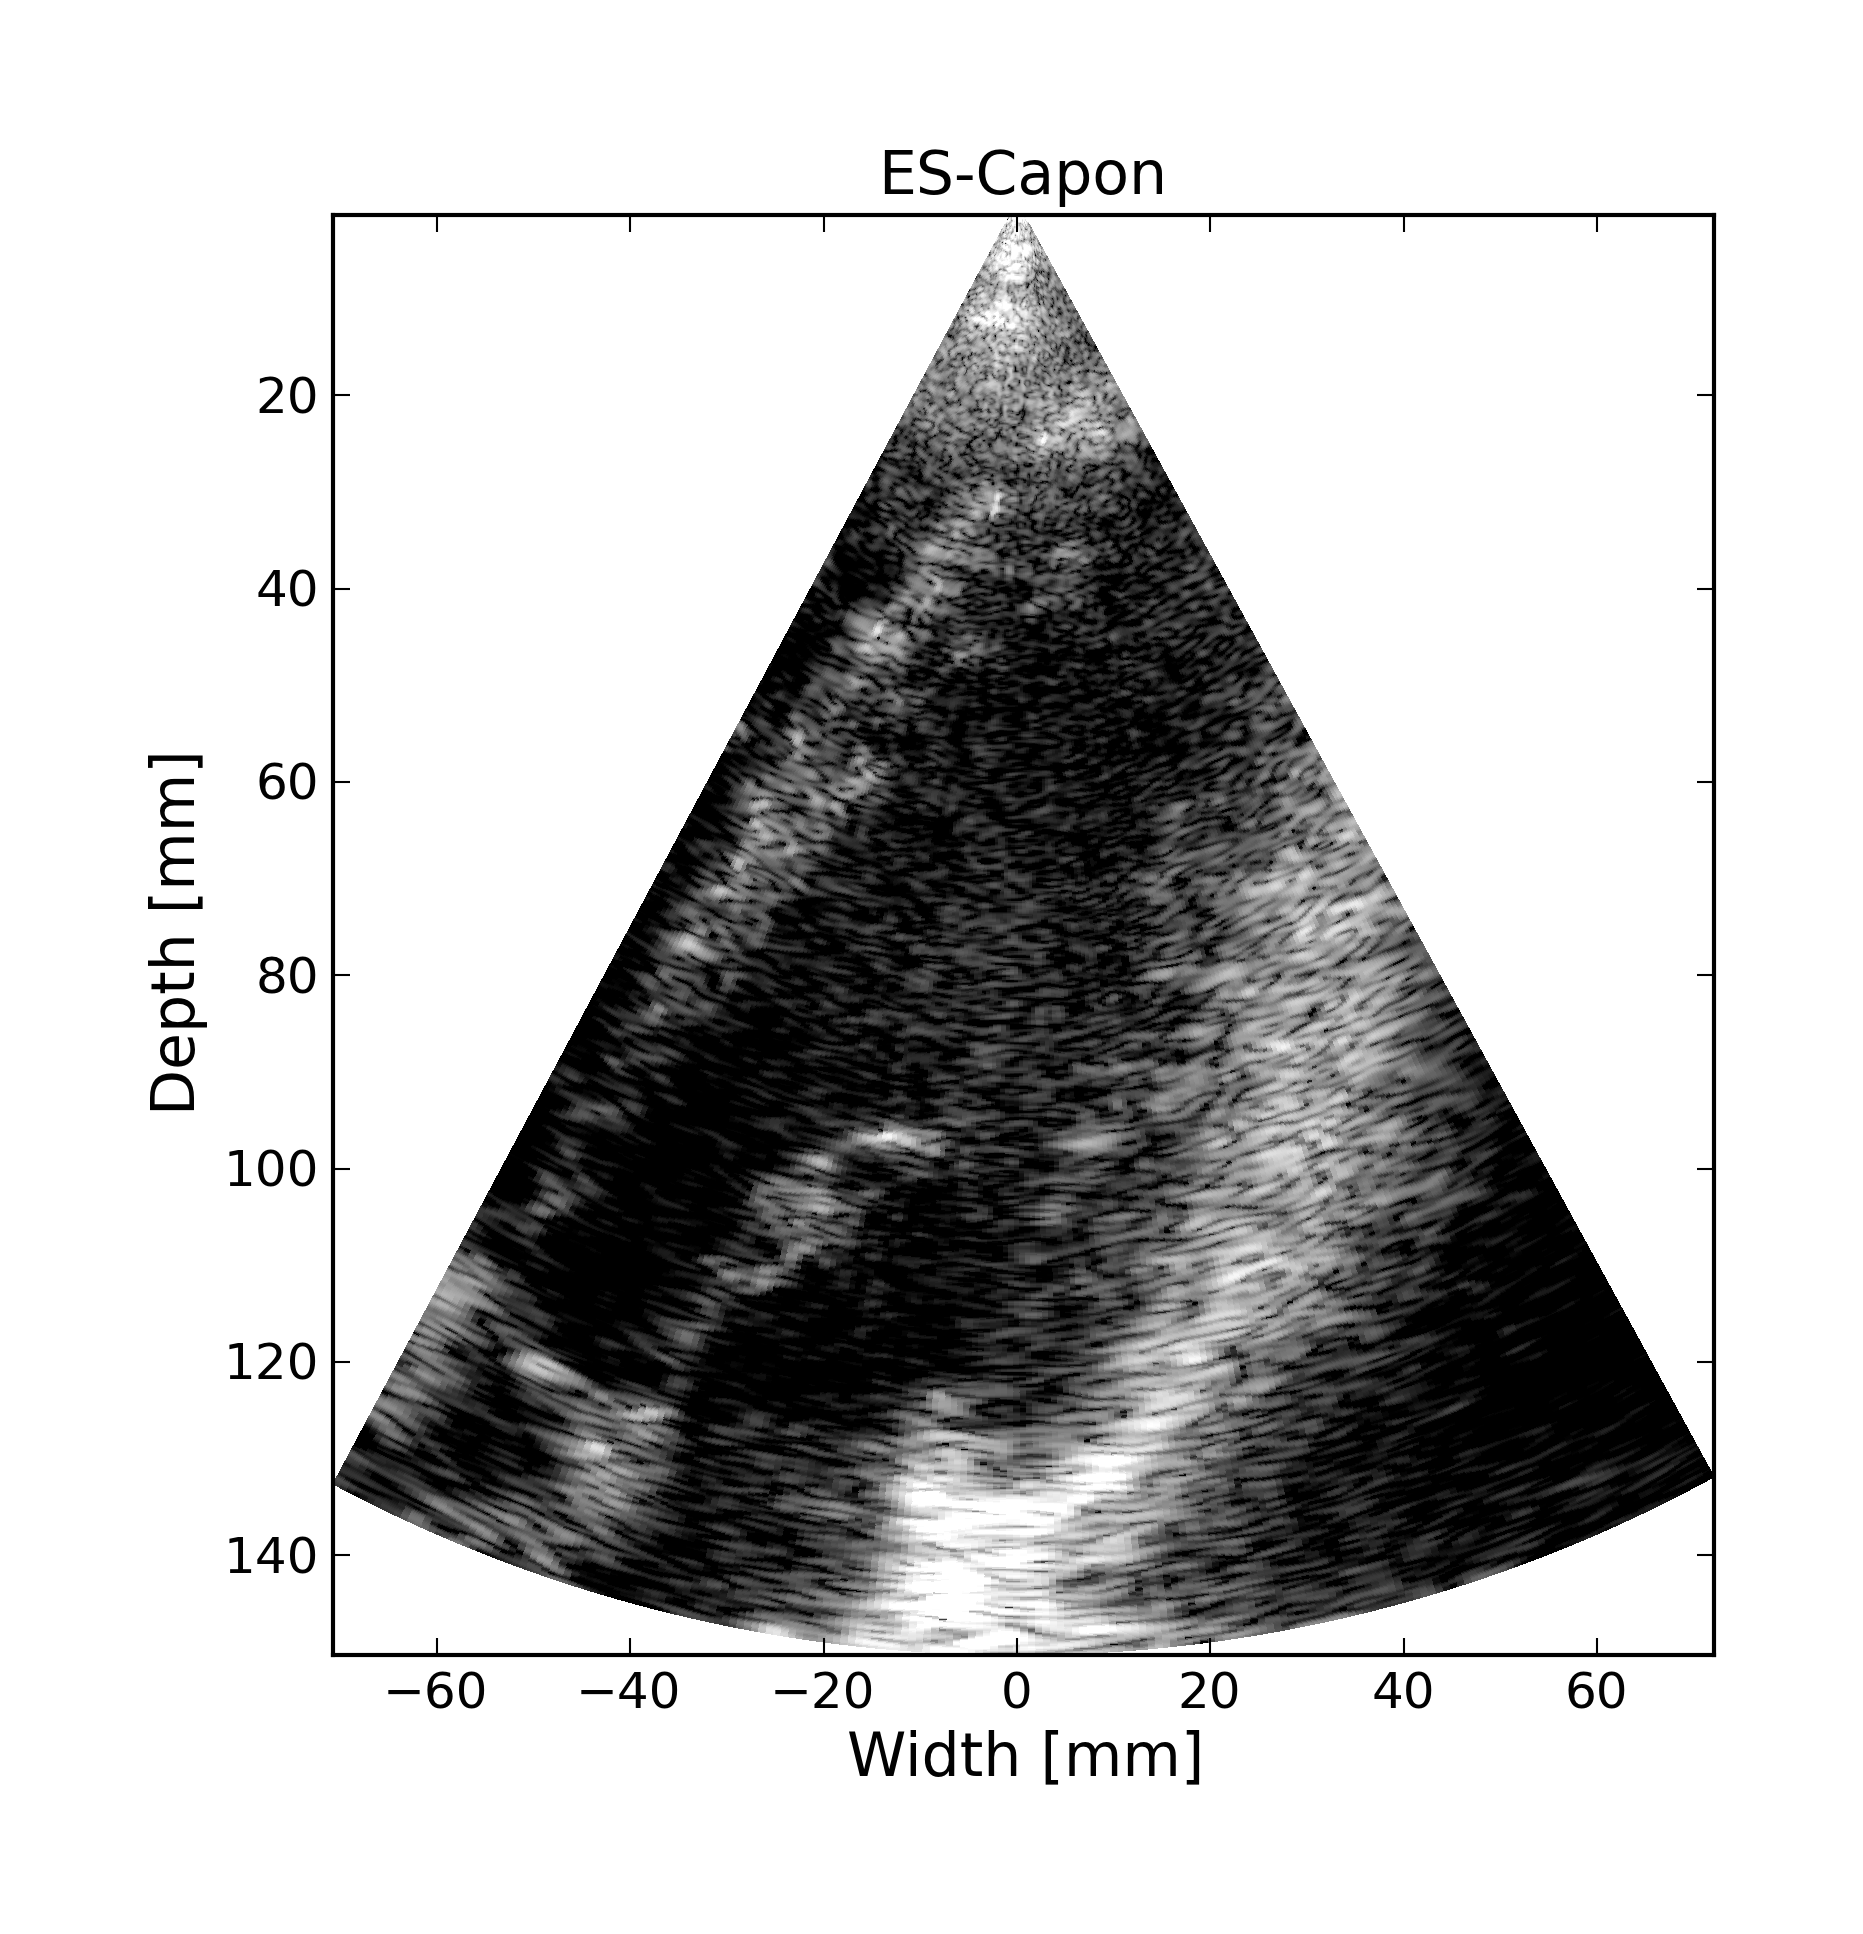
\includegraphics[width=2.2in]{gfx/capon_invivo.png} \label{fig:invivoMV}}
\hfil
\subfloat[]{
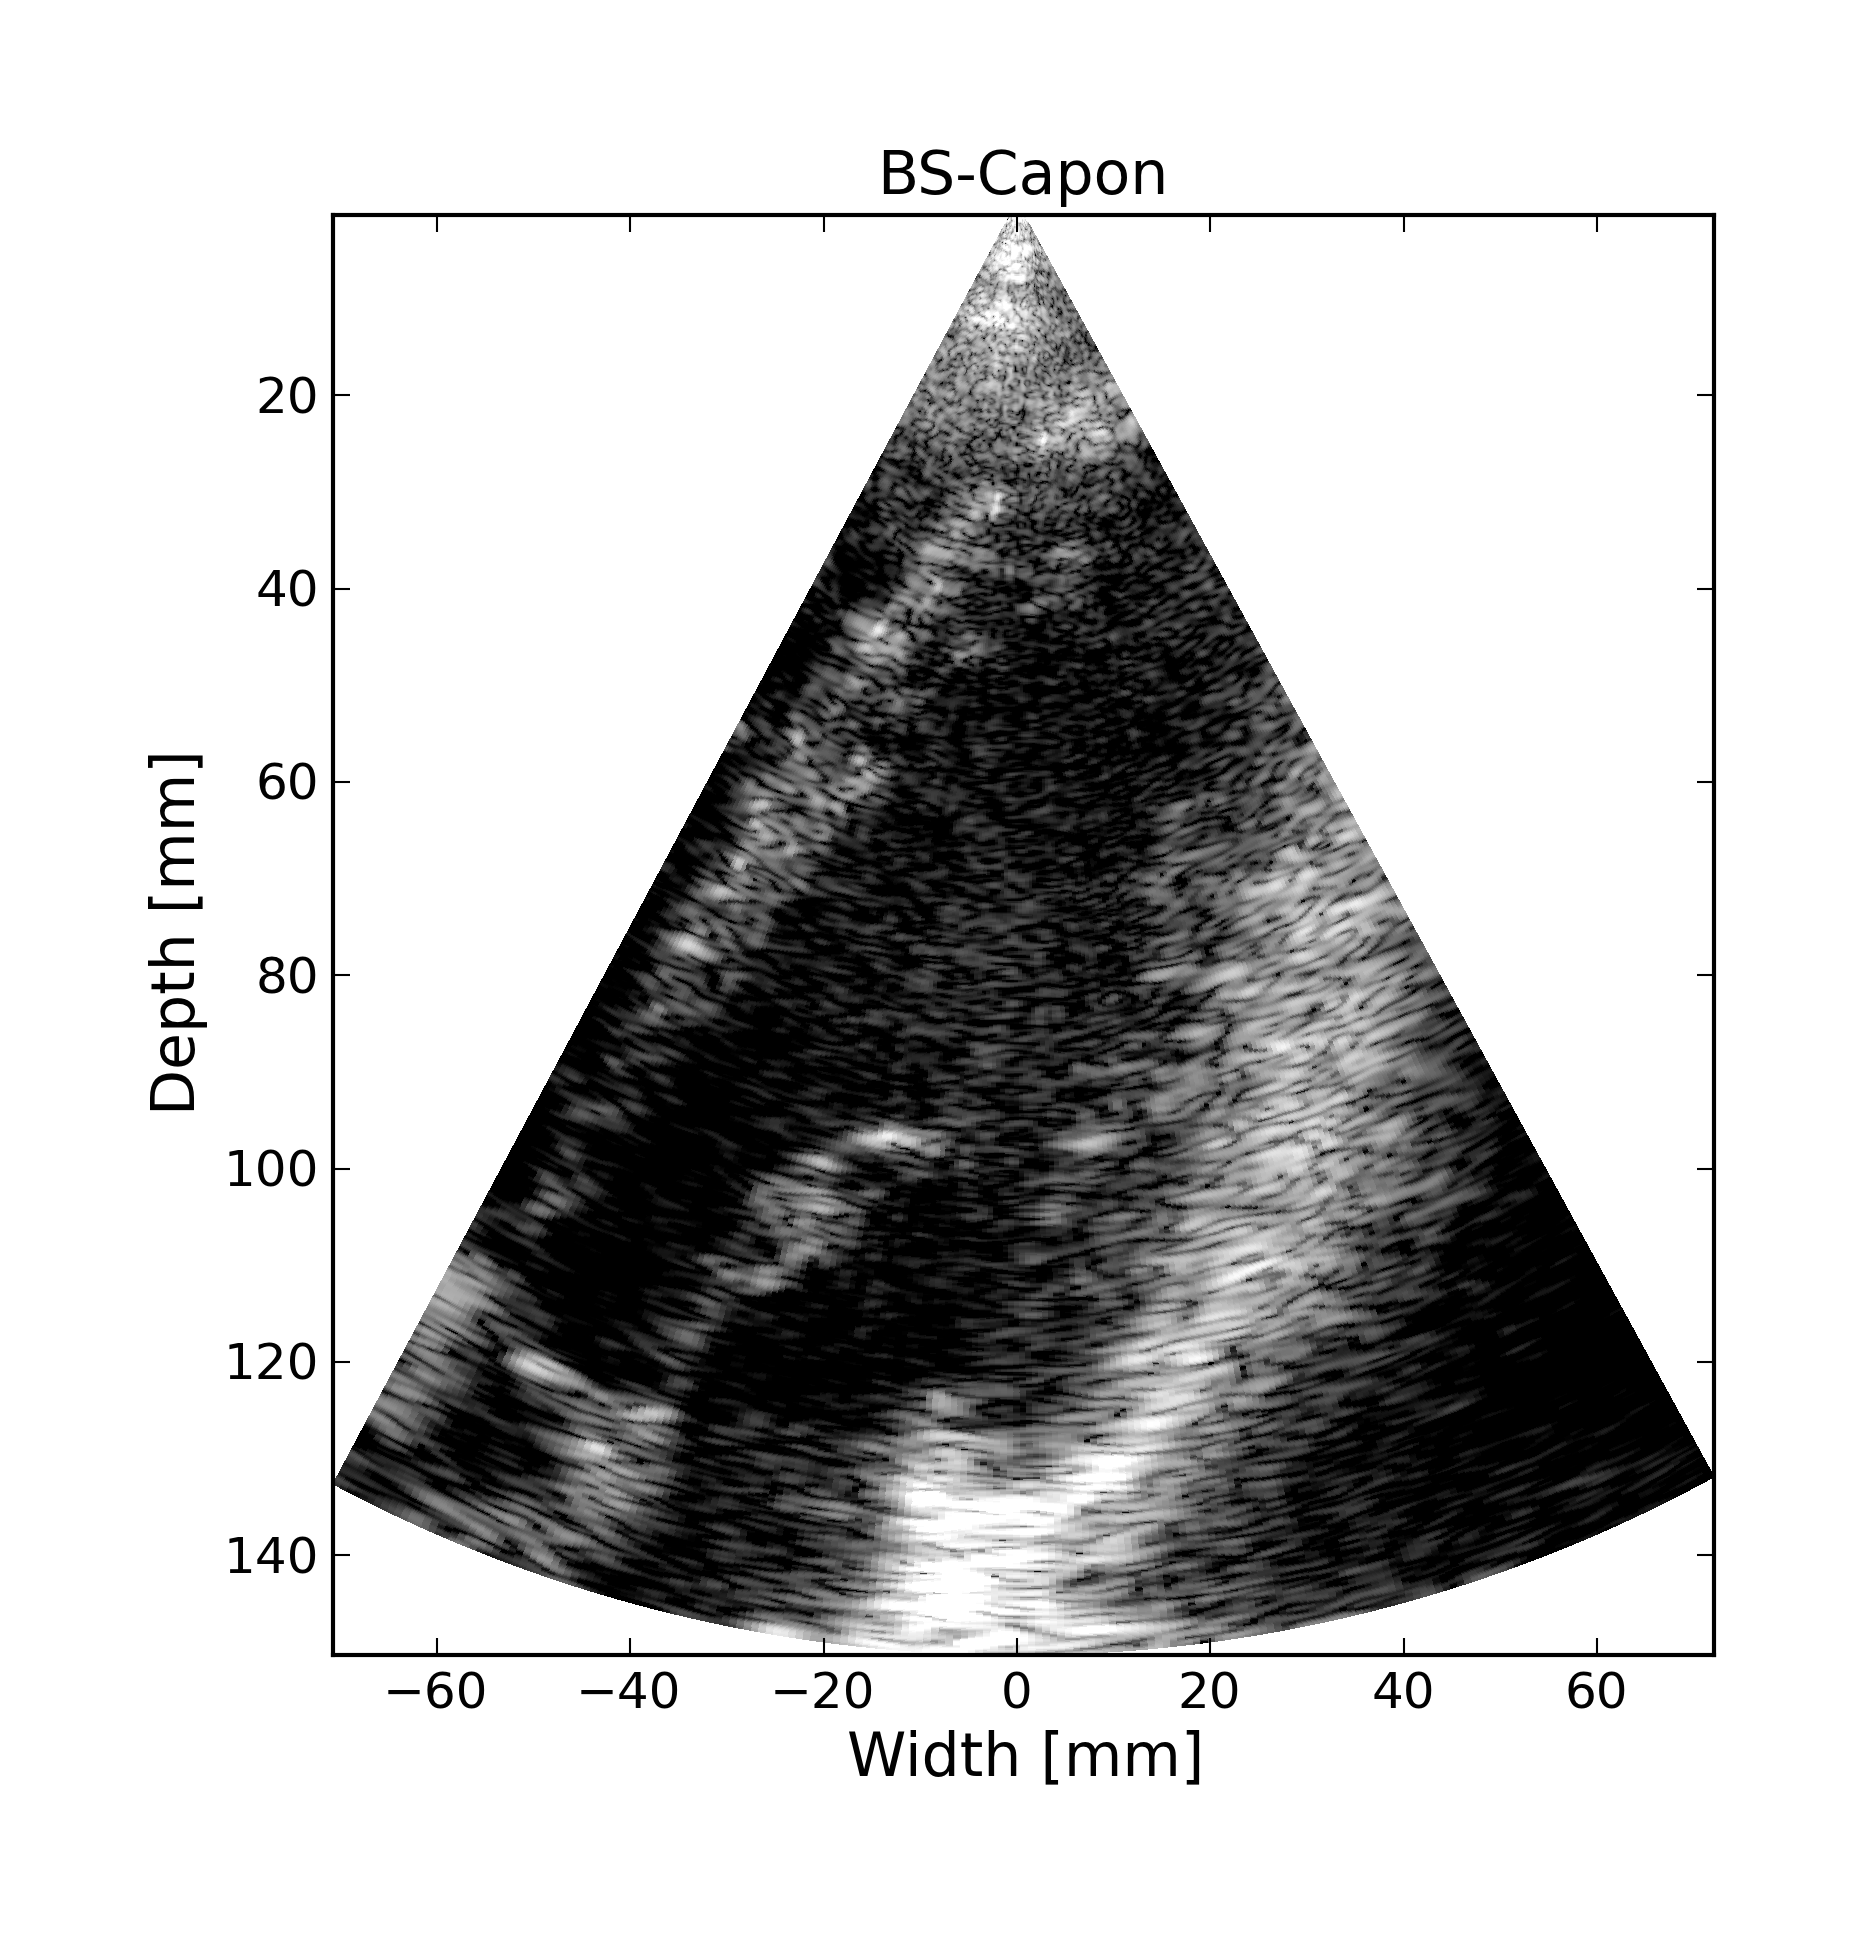
\includegraphics[width=2.2in]{gfx/capon_bs_invivo.png} \label{fig:invivoBS}}
\hfil
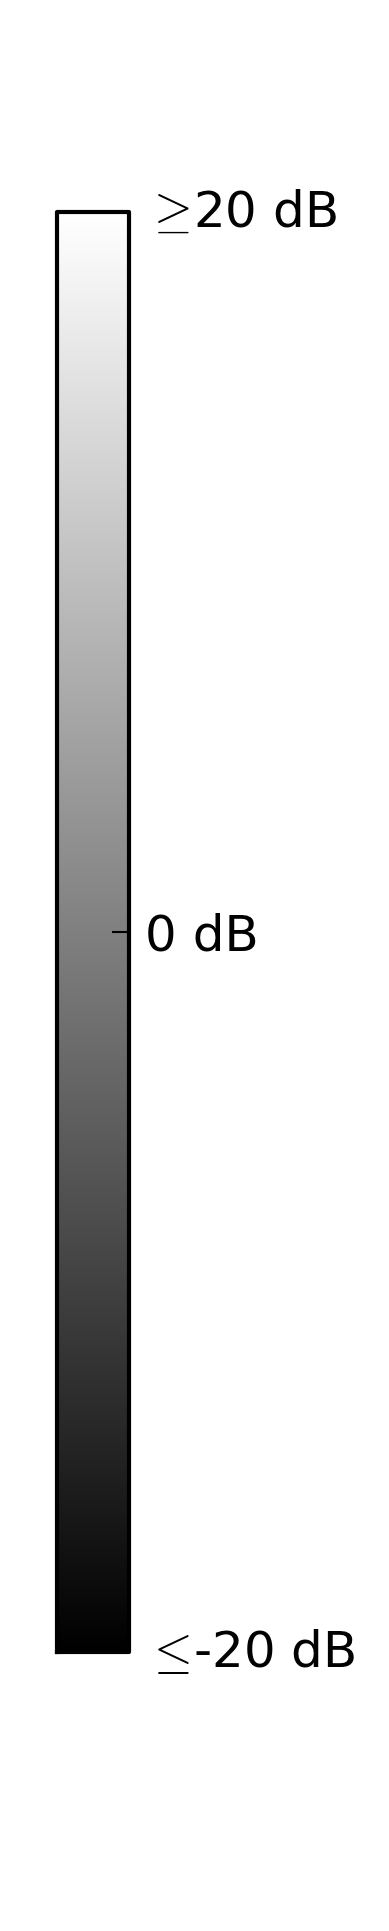
\includegraphics[width=0.4in]{gfx/colorBarInvivo2.png}
}
\caption{\textit{In-vivo} harmonic cardiac ultrasound image acquired using a 3.5 MHz, 64 elements phased array. Number of receive beams for the $70\degree$ sector is 98, and number of samples in range is 610. Dynamic range is -20 dB to 20 dB with mean value represented as 0 dB. The image is the first frame in the attached videos. a) Delay-and-sum with uniform weights \multimedia{Media-Movie 1}. b) Element-space Capon ($L=32, K=2, d=0.1$) \multimedia{Media-Movie 2}. c) Beamspace Capon ($L=32, K=2, N_b=3, d=0.01$) \multimedia{Media-Movie 3}.}
\label{fig:invivo}
\end{figure*}

%\begin{figure*}[!t]
%\centerline{
%\subfloat[]{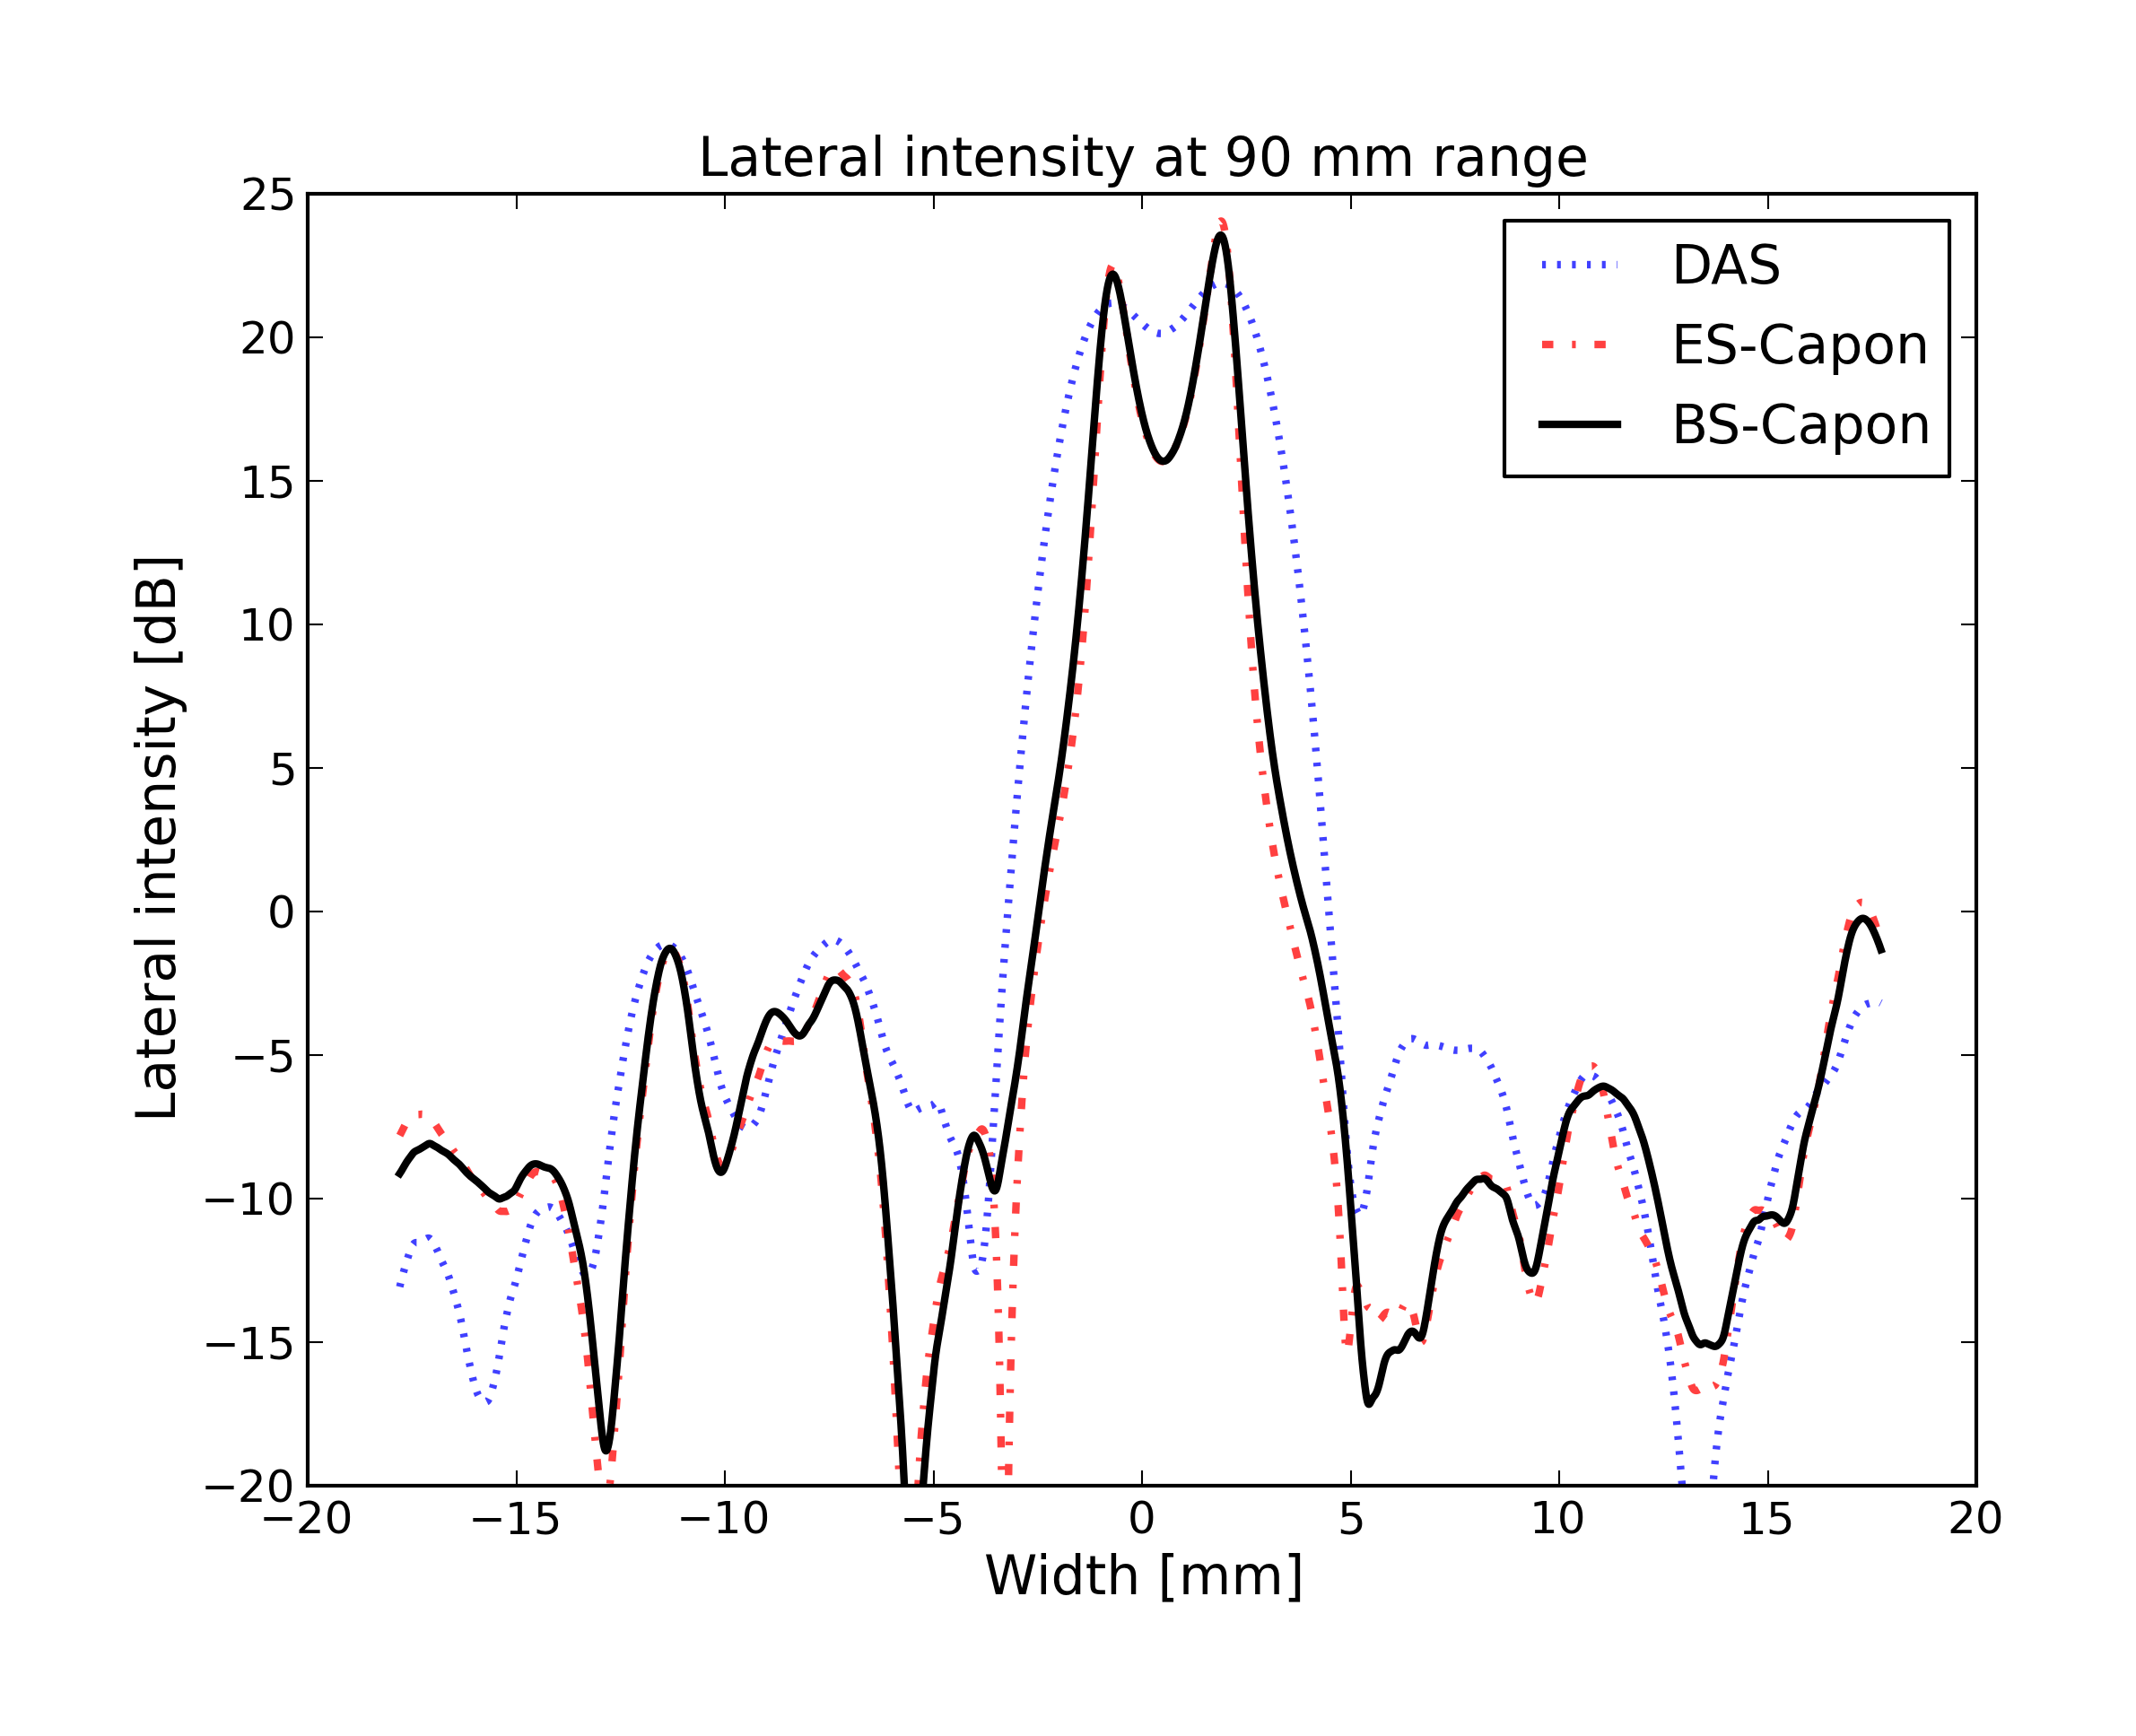
\includegraphics[width=3in]{gfx/simulation_slice.png} \label{fig:simulationSlice}}
%\hfil
%\subfloat[]{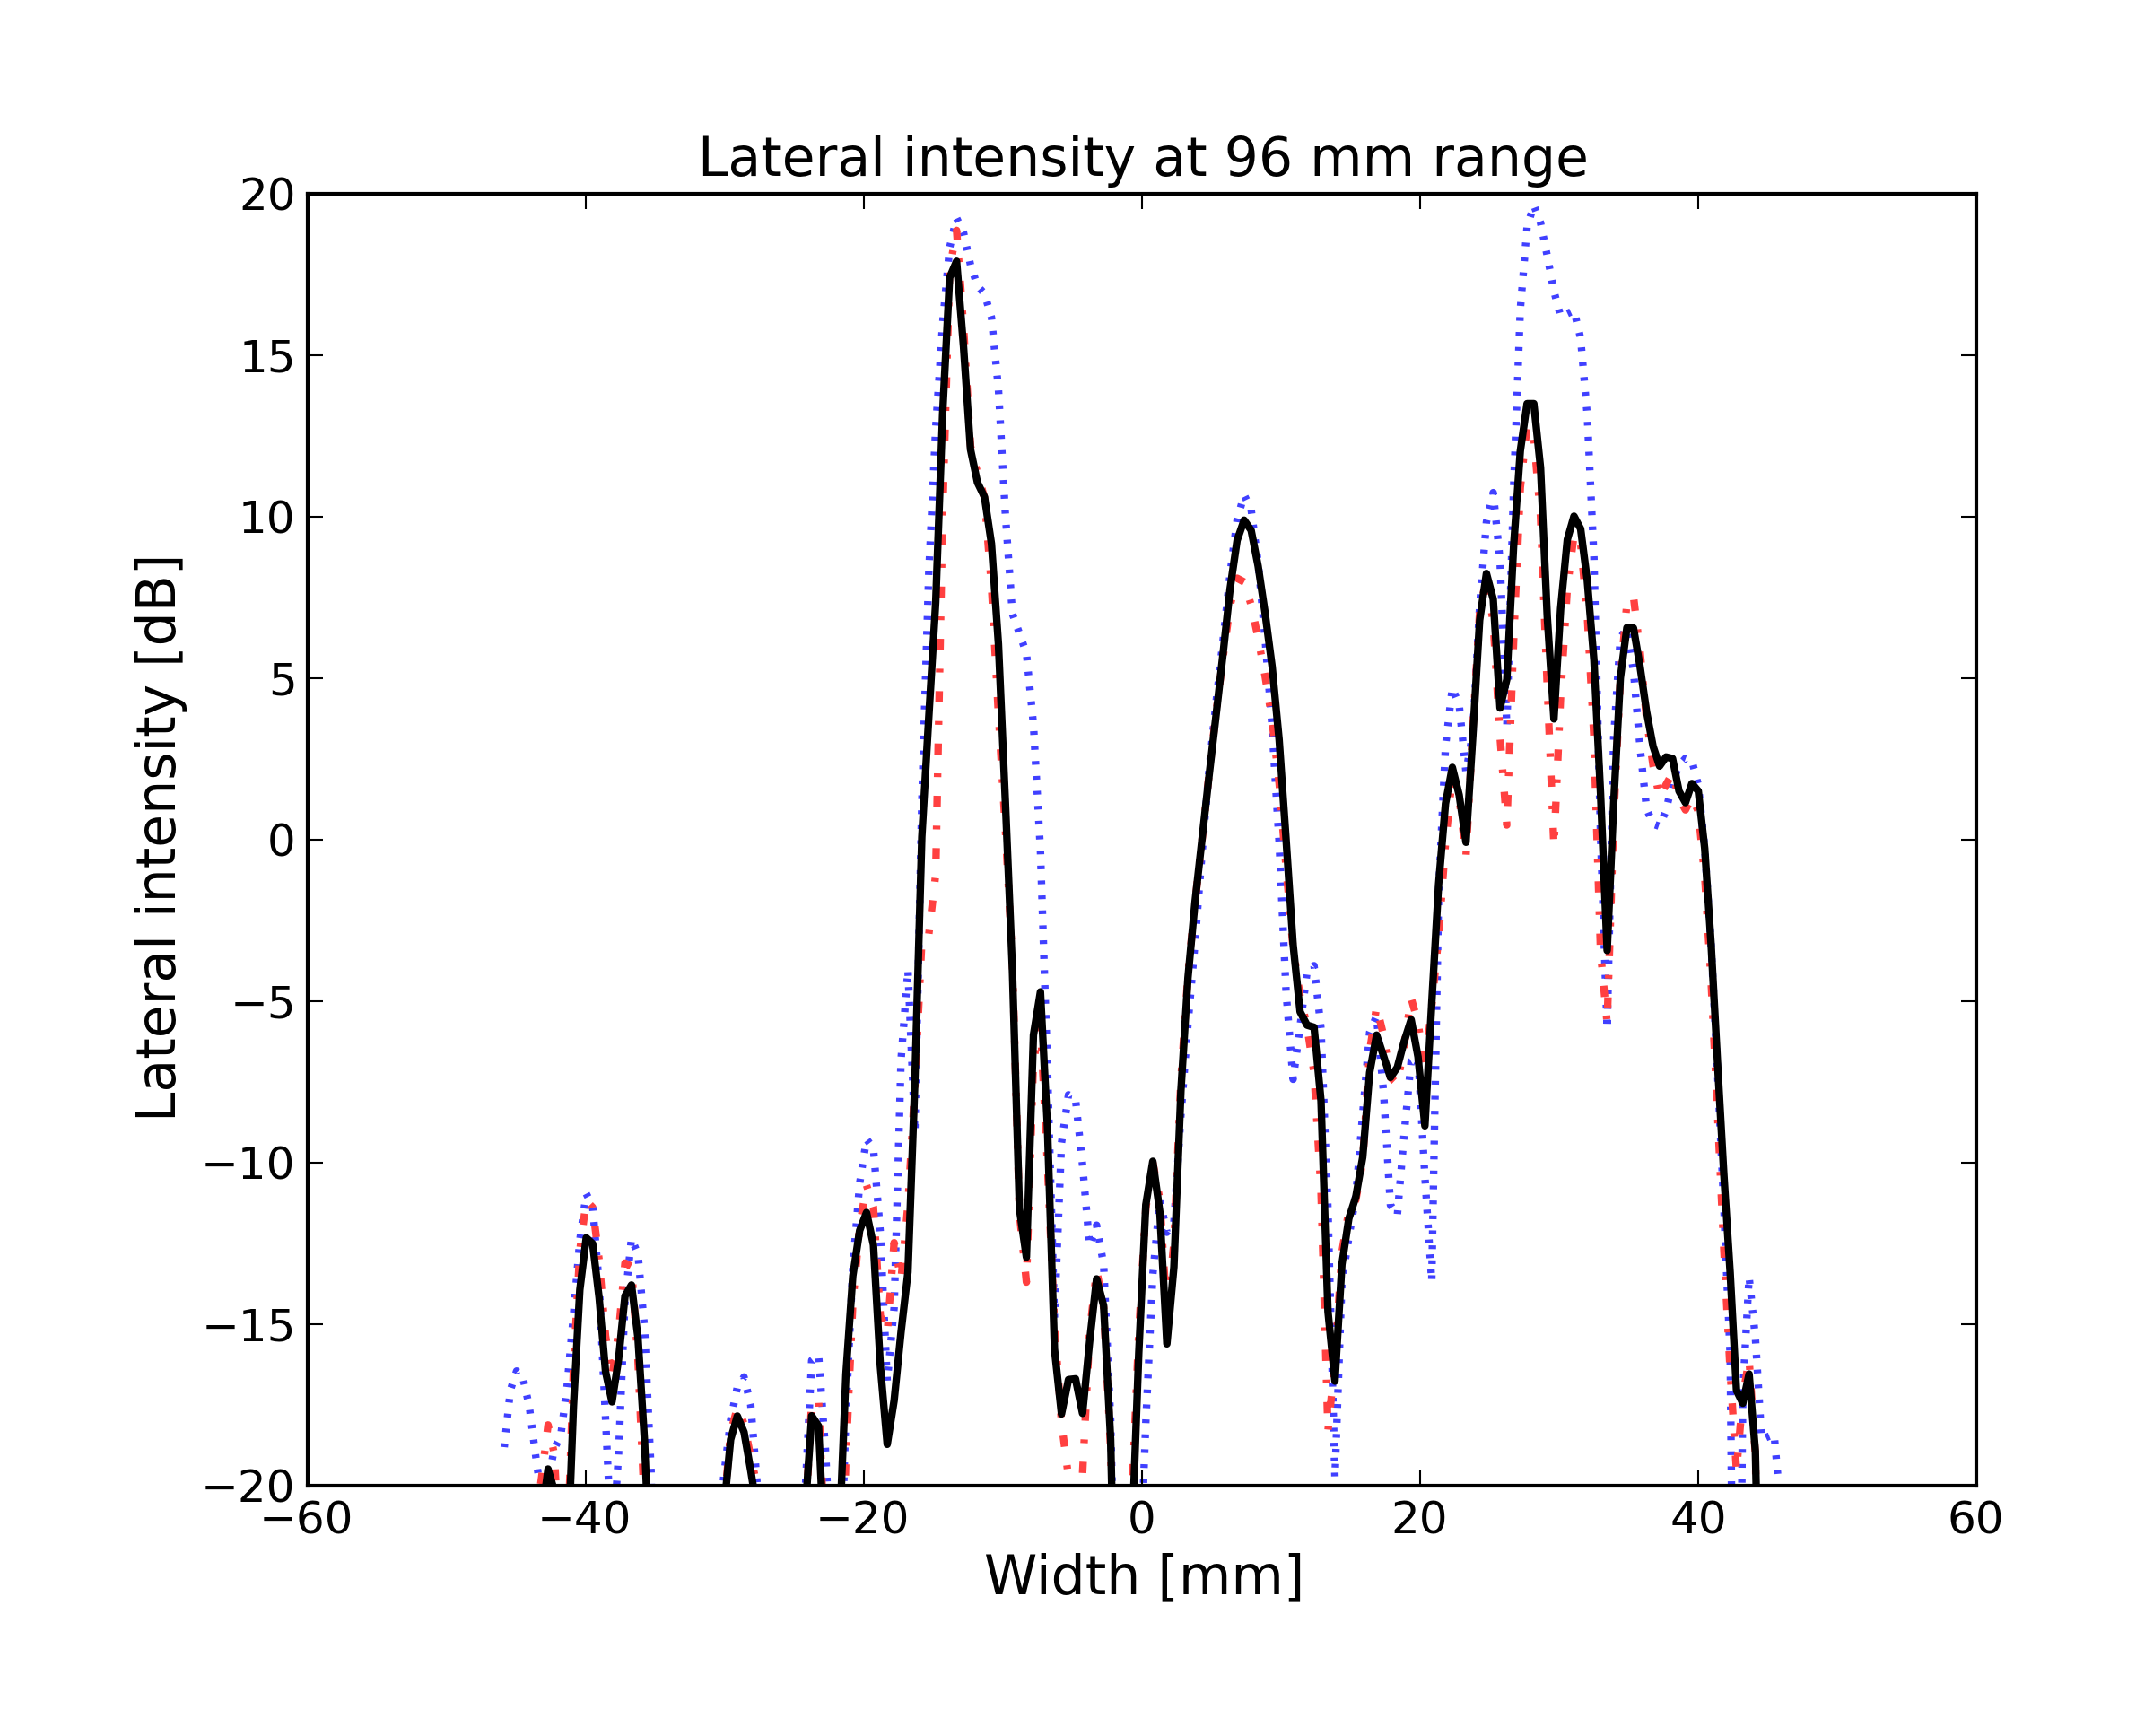
\includegraphics[width=3in]{gfx/invivo_slice.png} \label{fig:invivoSlice}}
%}
%\caption{Lateral slices taken from the images in Fig. \ref{fig:phantom} and Fig. \ref{fig:invivo}. a) From Fig. \ref{fig:phantom} at 93 mm constant depth, through the two bright point scatterers. b) From Fig. \ref{fig:invivo} at 96 mm range, through the tip of the mitral valve.}
%\label{fig:slices}
%\end{figure*}

%To investigate the image quality of both the ES and BS-Capon beamformer, a phantom was simulated using Field II \cite{Jensen1992, Jensen1996a} (Fig. \ref{fig:phantom}). The simulation was performed using a 64-element, $p=\lambda/2$ pitch, 10 $\mu$m kerf, 80\% bandwidth, and 10 mm high phased array. The transducer was excited with a 3.4 MHz and $1.5\lambda$ long pulse with transmit focus at 90 mm. The phantom contains two circular areas, one bright at 20 dB and one dark at -20 dB, and two point targets at 30 dB, located at 90 mm depth. Speckle level is at 0 dB, covering an area from $\pm90\degree$ in azimuth. The resulting image has been processed both using DAS with uniform weights, ES- and BS-Capon. The presented image is frame $15$ in a series of images where motion is imposed on both circles, point targets and the probe. The entire simulation is presented in two attached videos \multimedia{Media-Movie 1 and 2}.

Fig.\ \ref{fig:invivo} presents results of applying ES- and BS-Capon on an \textit{in-vivo} image of the left ventricle. The image was acquired using a 64-element and $p=0.65\lambda$ pitched phased array in harmonic mode (1.7 MHz at transmit and 3.4 MHz at receive). The image frame is extracted from a cardiac cycle, that can be viewed in its full length in the attached videos \multimedia{Media-Movie 1, 2 and 3}.
The region of interest is 70\degree{} with a minimal lateral sampling of 98 receive beams given by (\ref{eq:rayleigh}).
The image was acquired using 50 transmit beams and "Synthetic Transmit Beamforming" was used on receive \cite{Hergum2007}.  %It is included to show that both ES-Capon and BS-Capon beamforming are feasible for \textit{in-vivo} cardiac imaging, not just in simulations.

%To get a better impression of the improved lateral resolution obtained with Capon beamforming, two slices taken from the images in Fig. \ref{fig:phantom} and \ref{fig:invivo} are included in Fig. \ref{fig:slices}. For the phantom, the cut goes through the two point targets at 90 mm constant radius, and for the cardiac image it goes through the tip of the mitral valve at 96 mm constant radius.

%Both data sets have 
The data set has been processed with the following settings for the ES-Capon beamformer: $L = 32$, $K = 2$, and $d=0.1$. These settings have previously been shown to provide improved lateral resolution while maintaining DAS-like speckle \cite{Synnevag2007a}. For BS-Capon the following parameters have been used: $L=32$, $K=2$, $d=0.01$, and $N_b=3$. 

%When the simulated phantom was processed with the ES-Capon beamformer, modulation effects were observed when the two bright point scatterers moved across receive-beams. The artifact did not disappear until 16x lateral oversampling relative to (\ref{eq:rayleigh}) was used on transmit. 
%The cardiac recording shows a 70\degree{} sector with a minimal lateral sampling of 98 receive beams given by (\ref{eq:rayleigh}). %Despite this, the same artifacts were not observed here. 
%The image was acquired using 50 transmit beams and "Synthetic Transmit Beamforming" was used on receive \cite{Hergum2007}. 

\section{Trading resolution for speed}\label{sec:trade}
As seen from Fig.\ \ref{fig:bench} the execution time, for the solver in particular, is reduced when $L$ is reduced. The same is true when $N_b$ is reduced in beamspace. So to gain an  increase in processing throughput we can reduce $L$ in element space or $N_b$ in beamspace. In this section we investigate how adjusting $L$ for ES-Capon and $N_b$ for BS-Capon impacts the lateral resolution. 

In Fig.\ \ref{fig:speed_res_trade}, the minimum distance between two point targets (while preserving a 6 dB saddle point in between the two) is plotted against $L$ (when processed with ES-Capon) and $N_b$ (when processed with BS-Capon). To produce the result in Fig.\ \ref{fig:speed_res_trade} $K=2$ and $d=0.01$ has been used on both methods in order to obtain the same resolution for $L=N_b=M/2$. 
In Fig.\ \ref{fig:invivo}, the diagonal loading factor for BS-Capon was adjusted to make the two results equal for $L=32$ and $N_b=3$. %The resolution for ES-Capon is therefore better here than what is presented in Fig. \ref{fig:phantom}. 
%We considered this to be a small value for ES-Capon and a normal value for BS-Capon (cf. Section \ref{sec:bs}), hence the resolution for ES-Capon is here better than what is presented in Fig. \ref{fig:phantom}.

The phantom used contained two point targets with 30 dB amplitude located at 90 mm depth. The two point targets were placed inside speckle, with 0 dB in amplitude, covering an area from $\pm90\degree$ in azimuth. The phantom was simulated using Field II \cite{Jensen1992, Jensen1996a}. The simulation was performed using a 64-element, $p=\lambda/2$ pitch, 10 $\mu$m kerf, 80\% bandwidth, and 10 mm high phased array. The transducer was excited with a 3.4 MHz and $1.5\lambda$ long pulse with transmit focus at 90 mm. The precision of the presented measurements is 0.12 mm, dictated by the simulated frame rate of 25 FPS, and the relative speed of the two point scatterers, 3 mm/s. To avoid having to deal with signal cancellation and errors caused by not hitting each point with a receive beam, 16x oversampling has been used on transmit. 

For high values of $L$ and $N_b$ the two methods are equal, but for lower values, BS-Capon provides improved resolution compared to using small subarrays. We see that the resolution for BS-Capon gradually decreases due to an automatic increase in diagonal loading (cf. end of Section \ref{sec:bs}). If we compensate by reducing $d$, BS-Capon will provide resolution equal to ES-Capon (with $L=M/2$) for all values of $N_b$ except one \cite{Nilsen2009}. For $N_b=1$ the resolution is worse than for DAS because of a triangular apodization caused by subarray averaging. 

In element space, resolution decays rapidly since the effective adaptive aperture is proportional to $L$. For $L = N_b=3$, BS-Capon provides almost 1 mm improved resolution over DAS and ES-Capon. However, note that the resolution of the Capon beamformers strongly depends on the image signal-to-noise ratio (SNR) and the choice of parameters. Thus, different SNR scenarios and choices of parameters will lead to different results. It is also worth noting that ES-Capon beamforming in this example performs worse than DAS for small values of $L$. For these small subarrays, the method is not able to steer zeros at each point target or accurately micro-steer the main lobe. Subarray averaging further impose a triangular or trapezoid apodization function, which leads to worse resolution if the introduced adaptivity can not compensate for the increase in main lobe width. For $L=1$ the ES-Capon is equal to DAS.

\begin{figure}
\centering
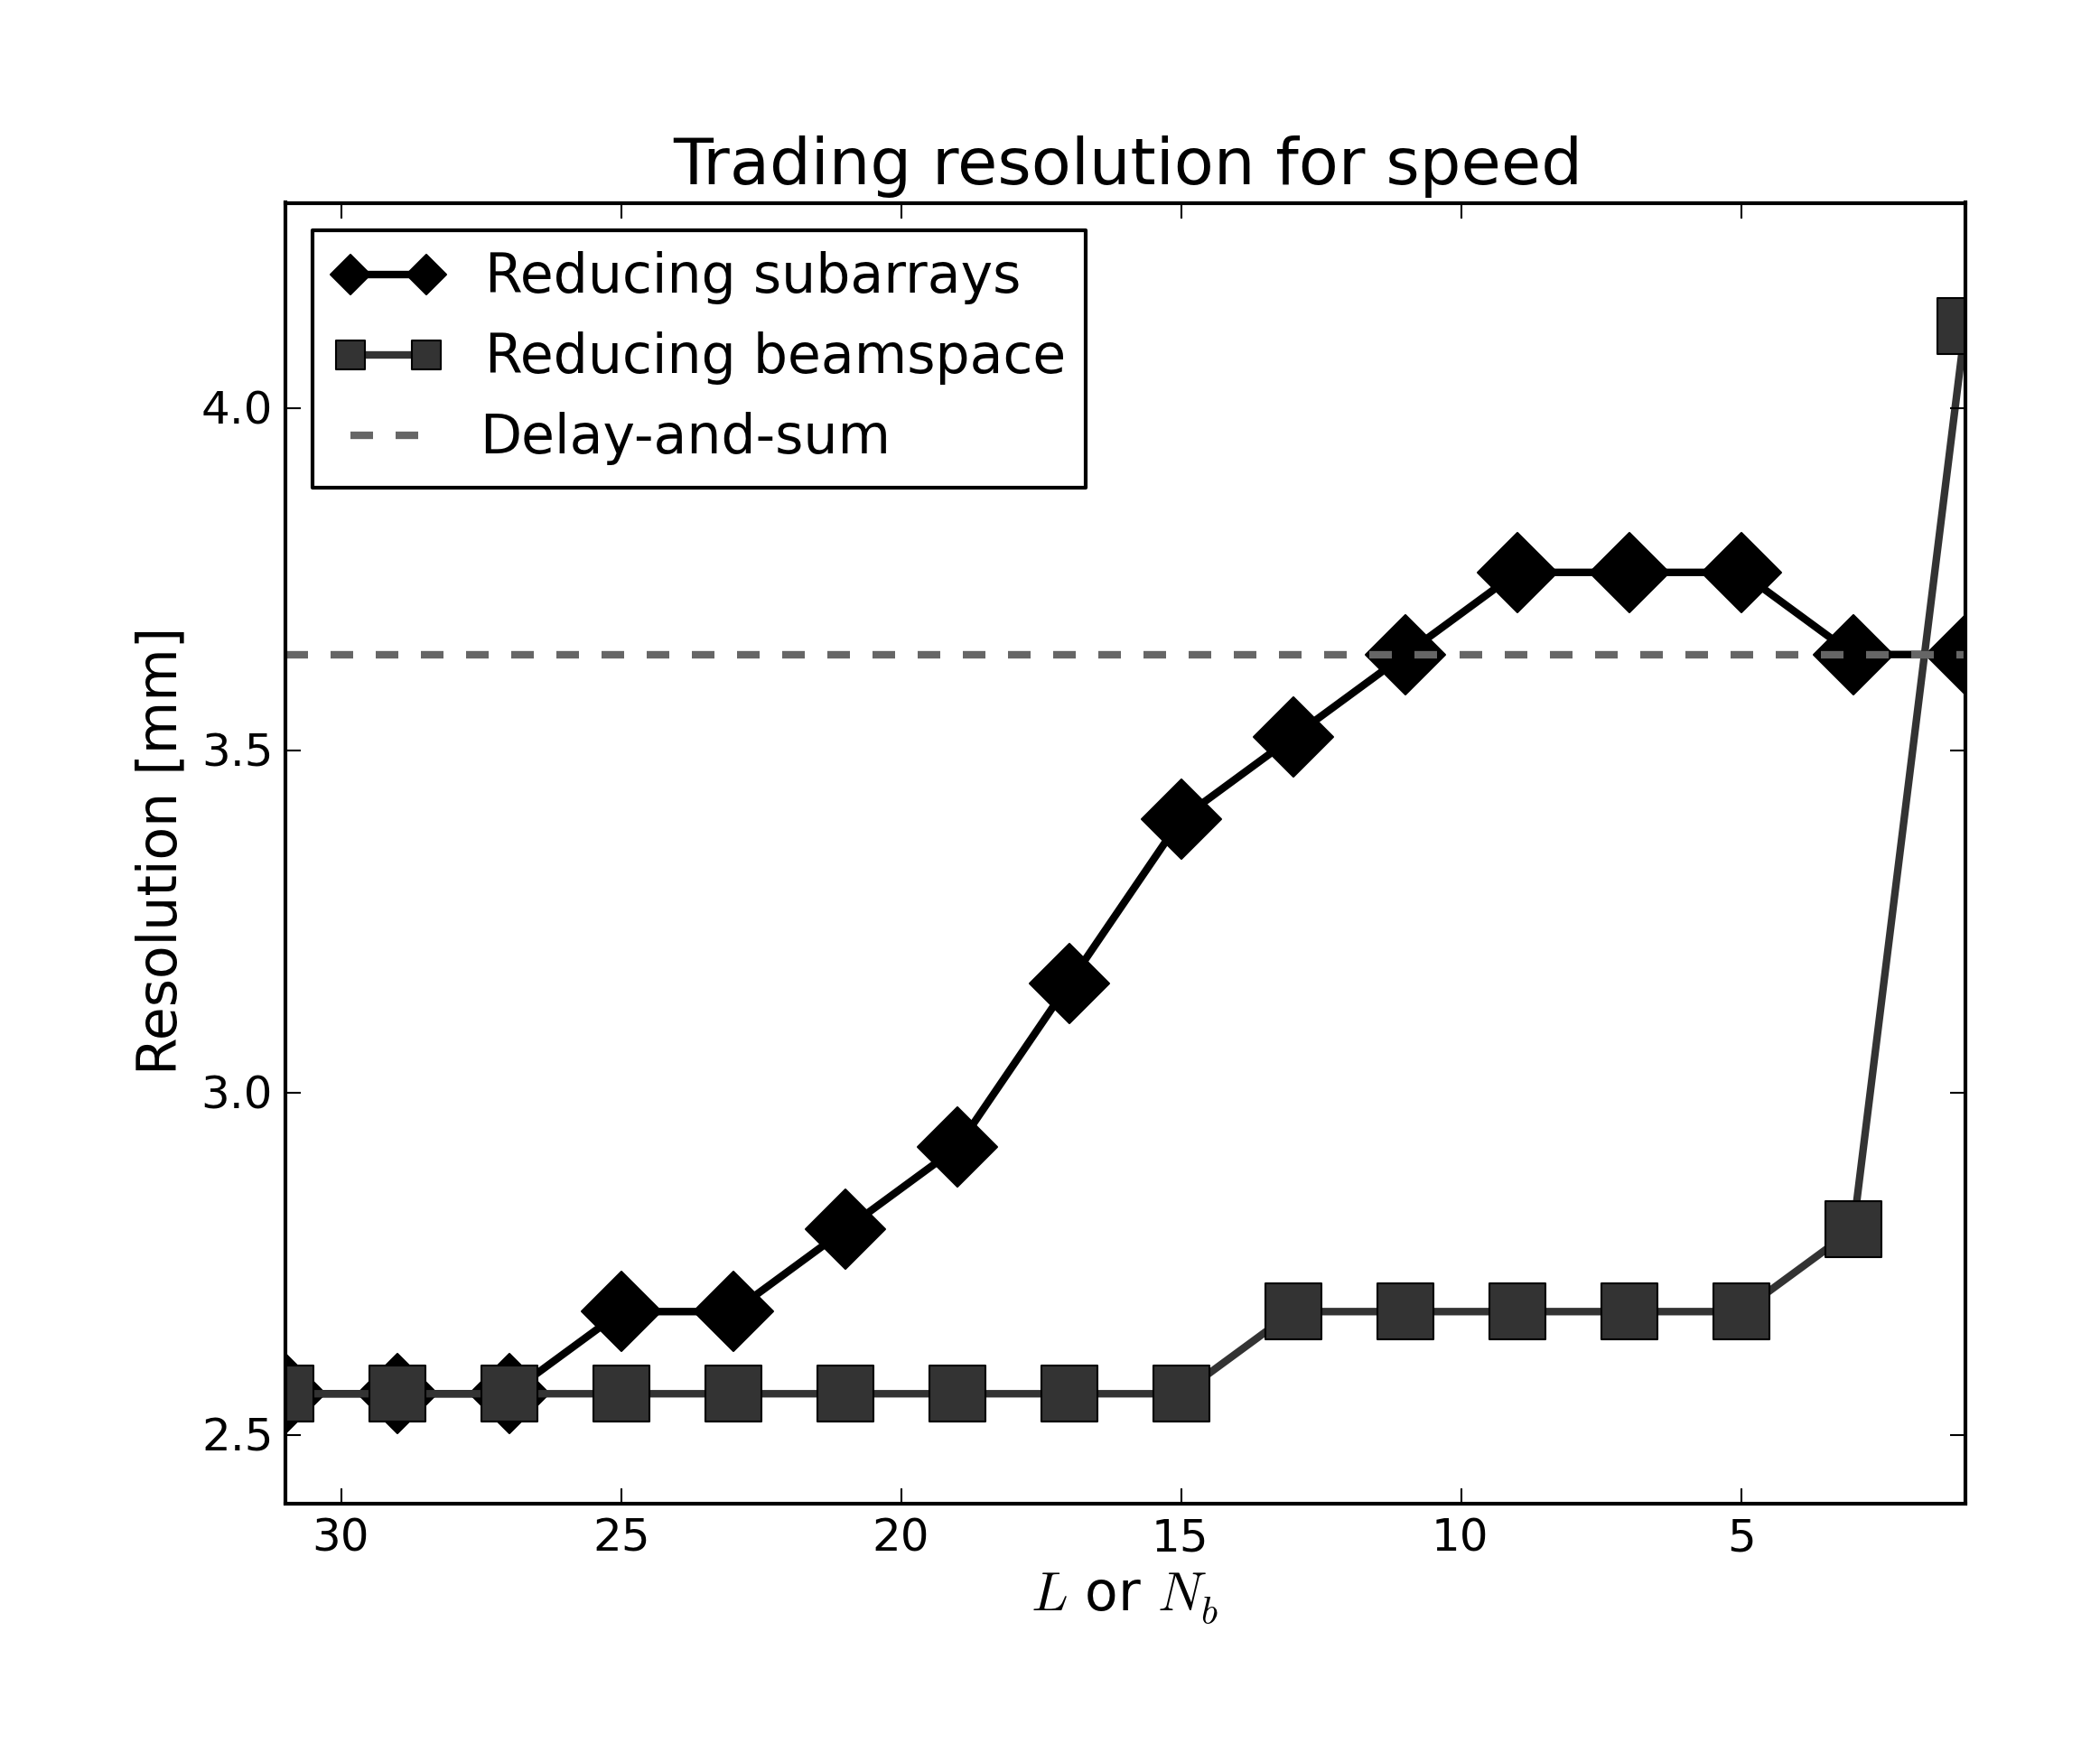
\includegraphics[width=3.3in]{gfx/speed_res_trade.png}
\caption{Trade-off between resolution and speed by reducing subarray size or reducing beamspace dimension. As $L$ or $N_b$ gets smaller, the execution time is reduced (Fig.\ \ref{fig:bench} and \ref{fig:benchBS}). When $N_b$ is varied, $L$ is fixed on 32.}
\label{fig:speed_res_trade}
\end{figure}

\section{Discussion}\label{sec:dis}
In this paper we have presented a parallel implementation of the BS-Capon beamformer for high-resolution cardiac ultrasound imaging. The results show that it is now possible to apply BS-Capon in real-time in cardiac ultrasound imaging by utilizing the power of a GPU. According to Fig.\ \ref{fig:benchBS} it is also possible to process two parallel receive lines per transmit beam (for both $M=64$ and $M=96$. $L=M/2$). %However, since we had to use oversampling in our simulation, these extra lines might be needed for increased sampling instead of increasing the frame rate. If parallel receive lines are used to obtain denser sampling, the acquisition time remains the same but the processing time is increased with a factor equal to the amount of oversampling. If parallel receive lines are used to increase the frame rate, the acquisition time is lowered, and the processing time remains constant. Hence, four parallel receive lines are not possible to process in real-time using BS-Capon with $N_b=3$ in combination with our single GPU setup.

For ES-Capon, processing rates for high quality settings are still too high to support real-time cardiac ultrasound imaging. From Fig.\ \ref{fig:benchUS64} we see that for $L = M/2 = 32$ and $K=1$, the total execution time is 110 ms (9 FPS). Taking into account that we use complex data, but less samples per image, these results are similar to the performance reported by Chen et al. \cite{Chen2011}.

A major part of the total execution time for ES-Capon comes from solving the system of linear equations. This limitation is targeted by reducing the sample covariance matrix size in beamspace, and as shown in Fig.\ \ref{fig:benchBS}, inverting the $3\times3$ beamspace covariance matrix is then barely visible. The time it takes to construct all covariance matrices is also reduced, but for few beams this is now the major contributor to the total execution time. If real-time is defined as 10 FPS \cite{Chen2011} almost all execution times in both Fig.\ \ref{fig:benchUS64} and \ref{fig:benchBS} are real-time. More natural for cardiac ultrasound imaging is to define real-time as the time it takes to acquire the underlying image. With this requirement the images formed using a 64 and 96 element array have a real-time requirement of 62.5 and 41.7 FPS respectively using single line acquisition. Each benchmark plot has a line indicating this real-time requirement. With beamspace processing, all processing times for large subarrays are below this line.

This paper further shows how to obtain a parallel formulation of the BS-Capon beamformer, and how to implement it in a GPU framework. The per-pixel granularity suggests that the beamformer is easily dividable across multiple GPUs. It is therefore possible to achieve higher frame rates if several GPUs are used simultaneously. However, there is usually a space-cost-energy limitation for how many GPUs that can be assembled in an ultrasound scanner.
 
%Turning to image quality we see from Fig. \ref{fig:phantom}, and the attached video of the simulation, that Capon beamforming provides improved lateral resolution of moving point targets both in element- and in a reduced beam-space ($N_b=3$). Our preliminary finding is that the Capon beamformers are local shift invariant as long as the lateral sampling is increased to a certain level in simulations \multimedia{Media-Movie 1 and 2}. %How large this oversampling factor needs to be and how the oversampling in the end is conducted will impact the real time requirement, and . 
%Future work should focus on how large this oversampling needs to be and how it should be conducted in order to still achieve real time processing.
%No major improvement in contrast is visually observed in the presented images and videos, other than slightly rounder circles due to mainlobe micro steering. 

Turning to image quality we see from Fig.\ \ref{fig:speed_res_trade} and the attached videos, that Capon beamforming provides improved lateral resolution of moving point targets both in element- and in a reduced beam-space ($N_b=3$). In the cardiac recording (Fig.\ \ref{fig:invivo}), structures are thinner and better resolved when the Capon beamformers are applied. One example is the mitral valve located at 10 cm depth and -1.5 cm width. On the other hand we observe a loss in contrast, especially in the septum (Fig.\ \ref{fig:invivo}, 6 cm depth, -2 cm width). This loss can be partially explained by the presence of highly correlated signals and mismatch between the assumed steering vector and signal. This is the same issue that made us use 16x oversampling when producing Fig.\ \ref{fig:speed_res_trade}. Future work should focus on how large this oversampling needs to be and how it should be conducted in order to still achieve real time processing.

In the end we want to point out that cardiac ultrasound has not been selected as the target modality in this paper because Capon beamforming shows large improvements in image quality in particular. It has been selected because it is the most computationally demanding modality, measured in floating points operations per second. The rationale being that if BS-Capon can run in real time for cardiac ultrasound it can run in real time for all medical ultrasound modalities. We believe that Capon beamforming may show more improvements in other imaging modalities where detection of small point targets is important.

%Nilsen and Hafizovic suggested to do automatic selection of beams in beamspace, hence picking the beams containing most energy. In this paper the center beams are always picked. This seems to work fine for focused systems, but an adaptive selection of beams should be implemented if interference at high angles is shown to contaminate the image.

%We expect that a large speedup had the Capon beamformer been implemented on the CPU using threads and SIMD (single instruction multiple data) instructions. 

%For a typical cardiac ultrasound image of 80*400 pixels (70 degree sector, 15cm range) acquired using a 2.5MHz, $M=64$ element phased array, the result is 10fps (subarray length $L=M/2$, temporal smoothing over 3 samples). If we do a 2-element pre-beamforming to get the channel count down to 32, the rate increases to 44fps. For a 32 element phased array we need less beams to cover the sector ($40 \times 400$ pixels), hence with the same parameters the frame rate increases to 87fps. The bottleneck of the Capon algorithm is to find the inverse covariance matrix for all pixels. This is an $O(L^3)$ operation, and results show that when L is larger than 16, real time performance is not possible for cardiac imaging with current high-end hardware. The target GPU has been Nvidia’s Quadro 6000, capable of 1Tflops.

\section{Conclusion}\label{sec:con}
In this paper a parallel formulation and implementation of the beamspace Capon beamformer have been presented, and
the beamformer has successfully been implemented on the GPU. For a three dimensional beamspace, processing rates supporting real-time cardiac ultrasound imaging was shown to be possible, meaning that processing rates higher than the image acquisition rate are obtained for a wide range of parameters. Image quality was investigated in an \textit{in-vivo} cardiac dataset. These results showed that Capon beamforming is feasible for cardiac ultrasound imaging, providing images with improved lateral resolution both in element- and beamspace.

%\section{Future work}
%Study shift invariance and minimum sampling...

%MLA's has, to some extent been used to increase later sampling. When using a high resolution beamformer, Nyquist tells us that the sampling frequency must be increase. Future work will concentrate on how much over sampling is required when using the Capon beamformer whit i curtain set of parameters...

%Plane waves...

% An example of a floating figure using the graphicx package.
% Note that \label must occur AFTER (or within) \caption.
% For figures, \caption should occur after the \includegraphics.
% Note that IEEEtran v1.7 and later has special internal code that
% is designed to preserve the operation of \label within \caption
% even when the captionsoff option is in effect. However, because
% of issues like this, it may be the safest practice to put all your
% \label just after \caption rather than within \caption{}.
%
% Reminder: the "draftcls" or "draftclsnofoot", not "draft", class
% option should be used if it is desired that the figures are to be
% displayed while in draft mode.
%
%\begin{figure}[!t]
%\centering
%\includegraphics[width=2.5in]{myfigure}
% where an .eps filename suffix will be assumed under latex, 
% and a .pdf suffix will be assumed for pdflatex; or what has been declared
% via \DeclareGraphicsExtensions.
%\caption{Simulation Results}
%\label{fig_sim}
%\end{figure}

% Note that IEEE typically puts floats only at the top, even when this
% results in a large percentage of a column being occupied by floats.


% An example of a double column floating figure using two subfigures.
% (The subfig.sty package must be loaded for this to work.)
% The subfigure \label commands are set within each subfloat command, the
% \label for the overall figure must come after \caption.
% \hfil must be used as a separator to get equal spacing.
% The subfigure.sty package works much the same way, except \subfigure is
% used instead of \subfloat.
%
%\begin{figure*}[!t]
%\centerline{\subfloat[Case I]\includegraphics[width=2.5in]{subfigcase1}%
%\label{fig_first_case}}
%\hfil
%\subfloat[Case II]{\includegraphics[width=2.5in]{subfigcase2}%
%\label{fig_second_case}}}
%\caption{Simulation results}
%\label{fig_sim}
%\end{figure*}
%
% Note that often IEEE papers with subfigures do not employ subfigure
% captions (using the optional argument to \subfloat), but instead will
% reference/describe all of them (a), (b), etc., within the main caption.


% An example of a floating table. Note that, for IEEE style tables, the 
% \caption command should come BEFORE the table. Table text will default to
% \footnotesize as IEEE normally uses this smaller font for tables.
% The \label must come after \caption as always.
%
%\begin{table}[!t]
%% increase table row spacing, adjust to taste
%\renewcommand{\arraystretch}{1.3}
% if using array.sty, it might be a good idea to tweak the value of
% \extrarowheight as needed to properly center the text within the cells
%\caption{An Example of a Table}
%\label{table_example}
%\centering
%% Some packages, such as MDW tools, offer better commands for making tables
%% than the plain LaTeX2e tabular which is used here.
%\begin{tabular}{|c||c|}
%\hline
%One & Two\\
%\hline
%Three & Four\\
%\hline
%\end{tabular}
%\end{table}


% Note that IEEE does not put floats in the very first column - or typically
% anywhere on the first page for that matter. Also, in-text middle ("here")
% positioning is not used. Most IEEE journals use top floats exclusively.
% Note that, LaTeX2e, unlike IEEE journals, places footnotes above bottom
% floats. This can be corrected via the \fnbelowfloat command of the
% stfloats package.



%\section{Conclusion}
%The conclusion goes here.





% if have a single appendix:
%\appendix[Proof of the Zonklar Equations]
% or
%\appendix  % for no appendix heading
% do not use \section anymore after \appendix, only \section*
% is possibly needed

% use appendices with more than one appendix
% then use \section to start each appendix
% you must declare a \section before using any
% \subsection or using \label (\appendices by itself
% starts a section numbered zero.)
%


%\appendices
%\section{Proof of the First Zonklar Equation}
%Appendix one text goes here.

% you can choose not to have a title for an appendix
% if you want by leaving the argument blank
%\section{}
%Appendix two text goes here.


% use section* for acknowledgement
\section*{Acknowledgment}
The authors would like to thank Prof. K. Kristoffersen, GE Vingmed Ultrasound and Norwegian University of Science and Technology, for valuable comments. 


% Can use something like this to put references on a page
% by themselves when using endfloat and the captionsoff option.
\ifCLASSOPTIONcaptionsoff
  \newpage
\fi



% trigger a \newpage just before the given reference
% number - used to balance the columns on the last page
% adjust value as needed - may need to be readjusted if
% the document is modified later
%\IEEEtriggeratref{8}
% The "triggered" command can be changed if desired:
%\IEEEtriggercmd{\enlargethispage{-5in}}

% references section

% can use a bibliography generated by BibTeX as a .bbl file
% BibTeX documentation can be easily obtained at:
% http://www.ctan.org/tex-archive/biblio/bibtex/contrib/doc/
% The IEEEtran BibTeX style support page is at:
% http://www.michaelshell.org/tex/ieeetran/bibtex/
\bibliographystyle{IEEEtran}
% argument is your BibTeX string definitions and bibliography database(s)
%\bibliography{IEEEabrv,../bib/paper}
\bibliography{mybib} % link to mendeley organized bibtex-file
%\bibliography{IEEEabrv,mybib} 
% <OR> manually copy in the resultant .bbl file
% set second argument of \begin to the number of references
% (used to reserve space for the reference number labels box)
%\begin{thebibliography}{1}

%\bibitem{IEEEhowto:kopka}
%H.~Kopka and P.~W. Daly, \emph{A Guide to \LaTeX}, 3rd~ed.\hskip 1em plus
%  0.5em minus 0.4em\relax Harlow, England: Addison-Wesley, 1999.

%\end{thebibliography}

% biography section
% 
% If you have an EPS/PDF photo (graphicx package needed) extra braces are
% needed around the contents of the optional argument to biography to prevent
% the LaTeX parser from getting confused when it sees the complicated
% \includegraphics command within an optional argument. (You could create
% your own custom macro containing the \includegraphics command to make things
% simpler here.)
%\begin{biography}[{\includegraphics[width=1in,height=1.25in,clip,keepaspectratio]{mshell}}]{Michael Shell}
% or if you just want to reserve a space for a photo:

% insert where needed to balance the two columns on the last page with
% biographies
%\newpage

\begin{IEEEbiography}[{\includegraphics[width=1in,height=1.25in,clip,keepaspectratio]{photos/jon_petter2.eps}}]{Jon Petter \AA{}sen}
(S12) was born in Porsgrunn, Norway in 1986. He received the B.Sc. and M.Sc. degree in computer science from the University of Oslo, Norway, in 2008 and 2010. He is currently pursuing his Ph.D. degree in medical ultrasound technology at the Norwegian University of Science and Technology (NTNU) Medical Imaging Lab (MI-Lab), Trondheim, Norway. 

He has industry experience from GE Vingmed Ultrasound, Horten, Norway, were he completed three summer internships from 2008 to 2010. His research interests include image and signal processing, adaptive ultrasound processing techniques and acceleration of ultrasound algorithms using Graphics Processing Units (GPUs). 
\end{IEEEbiography}

\begin{IEEEbiography}[{\includegraphics[width=1in,height=1.25in,clip,keepaspectratio]{photos/jo_inge2.eps}}]{Jo Inge Buskenes}
received the B.Sc. degree in electrical engineering from Gj\o{}vik College University, Norway, in 2007, and the M.Sc. degree in instrumentation for particle physics from the University of Oslo, Norway, in 2010. He is currently pursuing the Ph.D. degree in image reconstruction and technology at the University of Oslo.

His industry experience includes the European Organization for Nuclear Research (CERN), Geneva, Switzerland (2007-2008), and the Norwegian Defence Research Establishment, Kjeller, Norway (2009). He has lectured in digital signal processing at the Gj\o{}vik College University (2009), and at the University of Oslo (2010-2012). His research interests include adaptive beamforming, digital image reconstruction, high performance computing, intelligent detector design and embedded Linux platforms.
\end{IEEEbiography}

\begin{IEEEbiography}[{\includegraphics[width=1in,height=1.25in,clip,keepaspectratio]{photos/carl-inge.eps}}]{Carl-Inge Colombo Nilsen}
(S’06–M’10) received the M.Sc. and Ph.D. degrees in computer science from the University of Oslo, Norway, in 2005 and 2010. He is currently working at the University of Oslo as a postdoctoral research fellow. His research interests include signal and array processing for ultrasound imaging and other acoustic applications.
\end{IEEEbiography}

% insert where needed to balance the two columns on the last page with
% biographies
%\newpage

\begin{IEEEbiography}[{\includegraphics[width=1in,height=1.25in,clip,keepaspectratio]{photos/andreas.eps}}]{Andreas Austeng}
was born in Oslo, Norway, in 1970. He received the M.S. degree in physics in 1996 and the Ph.D. degree in computer science in 2001, both from the University of Oslo. Since 2001, he has been working at the Department of Informatics, University of Oslo, first as a postdoctoral research fellow and currently as an associate professor. His research interests include signal and array processing for acoustical imaging.
\end{IEEEbiography}

%\newpage

\begin{IEEEbiography}[{\includegraphics[width=1in,height=1.25in,clip,keepaspectratio]{photos/sverre.eps}}]{Sverre Holm}
(M’82-SM’02) was born in Oslo, Norway, in 1954. He received the M.S. and Ph.D. degrees in electrical engineering from the Norwegian Institute of Technology, Trondheim, in 1978 and 1982, respectively. His academic experience includes Yarmouk University in Jordan (1984-1986) and the Norwegian Institute of Technology and later the University of Oslo (1989-1994) as an adjunct professor. Since 1995, he has been a professor of signal processing in the Department of Informatics at the University of Oslo. In 2002, he was elected a member of the Norwegian Academy of Technological Sciences, and in 2009, he became an adjunct professor in the Norwegian University of Science and Technology (NTNU) Medical Imaging Lab, Trondheim. His industry experience includes GE Vingmed Ultrasound, Horten, Norway (1990-1994). He worked with Sonitor Technologies (2000-2005), where he developed ultrasonic technology that is the core of the indoor positioning system described in \textit{Scientific Americanin} 2008 as "a positioning system that goes where GPS can't." He has published about 130 publications internationally, plus about 10 patents. He has had sabbaticals at GE Global Research, NY (1998), and the Waves and 
Acoustics Laboratory of ESPCI, Paris (2008-2009). He was an associate editor of the \textit{IEEE Transactions on Ultrasonics, Ferroelectrics, and Frequency Control} from 1997 to 2002. His research interests are medical ultrasound imaging, modeling of tissue-ultrasound interaction, and ultrasound positioning.
\end{IEEEbiography}


% You can push biographies down or up by placing
% a \vfill before or after them. The appropriate
% use of \vfill depends on what kind of text is
% on the last page and whether or not the columns
% are being equalized.

%\vfill

% Can be used to pull up biographies so that the bottom of the last one
% is flush with the other column.
%\enlargethispage{-5in}



% that's all folks
\end{document}


